\chapter{Results and Analysis}
\label{ch:ResultsAnalysis}
In this chapter, the main objective is to present the findings from the experiments and analysis conducted in the previous chapters. The section is designed to show the performance of the trained models, especially focusing on the MLP regressor, which was trained on the COMB\textsubscript{synthetic} images. This chapter will include several tables, figures, and visualizations that show the results without going into detailed explanations. That will be covered in the next chapter. \par

\section{Label Distribution}
\label{sec:LabelDist}
The histograms in \autoref{fig:DistTestCriteria} for SCIN\textsubscript{authentic} and \autoref{fig:DistTestCriteria2} for SCIN\textsubscript{synthetic} show the spread and severity of distortions in the test datasets. Each histogram has five bins for each dermatology quality criterion. The first bin shows no distortion, and the other bins show increasing levels of distortion severity. \par
\begin{figure}[ht]
    \centering
    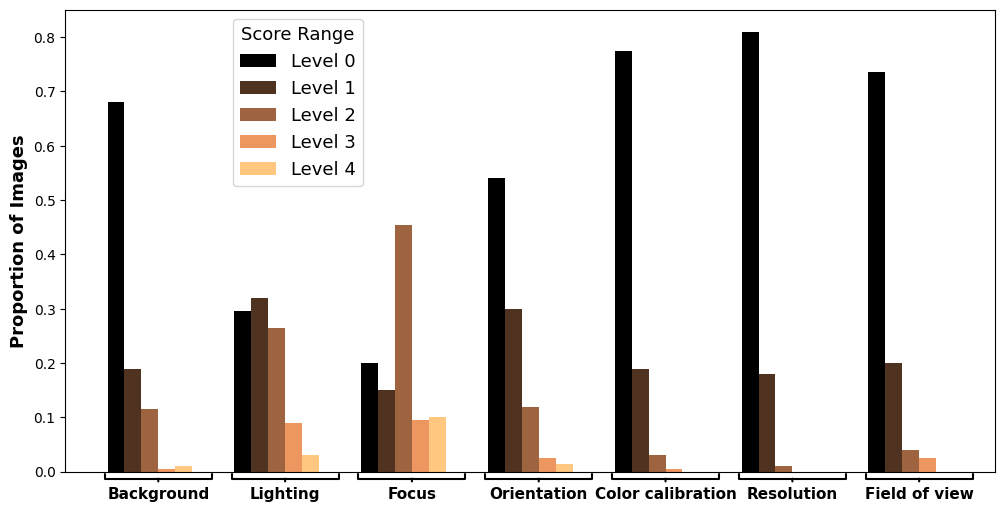
\includegraphics[keepaspectratio,width=15cm]{img/Distribution_test_criteria.png}
    \caption{Distribution of distortion scores for each dermatology quality criteria in the SCIN\textsubscript{authentic} test set. The histograms show the proportion of images at different levels of distortion severity, ranging from Level 0 (no distortion) to Level 4 (high distortion).}
    \label{fig:DistTestCriteria}
\end{figure}
\noindent
\clearpage
\autoref{fig:DistTestCriteria} shows the distribution of distortion scores for each dermatology quality criterion in the SCIN\textsubscript{authentic} test set. Most criteria are right-skewed, meaning higher levels of distortion are less common. However, focus and lighting have a more balanced spread of distortion levels.\par
\begin{figure}[ht]
    \centering
    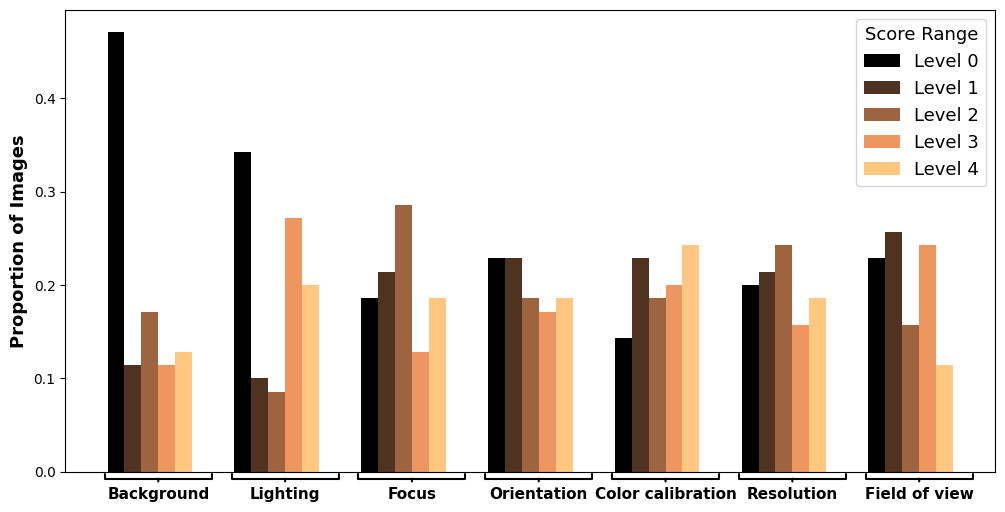
\includegraphics[keepaspectratio,width=15cm]{img/Distribution_test_criteria2.png}
    \caption{Distribution of distortion scores for each dermatology quality criteria in the SCIN\textsubscript{synthetic} test set. Unlike the SCIN\textsubscript{authentic} test set, these distributions are more balanced, showing that synthetic distortions were applied evenly across all severity levels.}
    \label{fig:DistTestCriteria2}
\end{figure}
\noindent
\autoref{fig:DistTestCriteria2} shows the distribution of distortion scores for each quality criterion in the SCIN\textsubscript{synthetic} test set. These distributions are more balanced, showing that the synthetic distortions were applied evenly across all severity levels. \par

\section{Visual Examples of Distortions}
\label{sec:DistPipeline}
The distortion pipeline is key to creating realistic image quality issues in the context of teledermatology. Each dermatology quality criterion includes multiple types of distortions, each with five levels of intensity. The distortions range from zero, meaning no distortion, to higher values that show increasing levels of the specified distortion. Visual examples of these distortions at different levels for each quality criterion are included in \autoref{sec:Degradation_Types}. These examples help to understand what each type of distortion looks like and how it impacts the images. \par

\clearpage
\section{Effect of Distortion Quantity on Performance}
\label{sec:DistQuant}
The scatter plots in \autoref{fig:NumDistReg} and \autoref{fig:NumDistCls} show how the overall Spearman Rank Order Correlation Coefficient (SRCC) changes with training time for different numbers of distortions. The points are colored based on the number of distortions in the dataset, helping to see how the size of the dataset affects model performance. \par

\begin{figure}[ht]
    \centering
    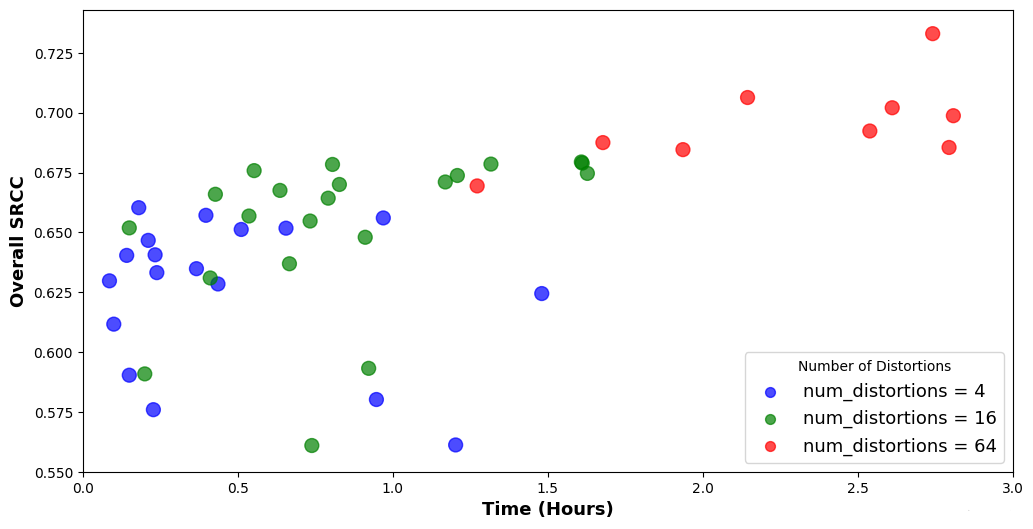
\includegraphics[keepaspectratio,width=13.5cm]{img/num_dist_reg.png}
    \caption{Overall SRCC for XGB Regressor and MLP Regressor with different numbers of distortions. The x-axis shows the training time, and the y-axis shows the SRCC values. Larger datasets generally lead to better performance but take more time to train.}
    \label{fig:NumDistReg}
\end{figure}
\begin{figure}[ht]
    \centering
    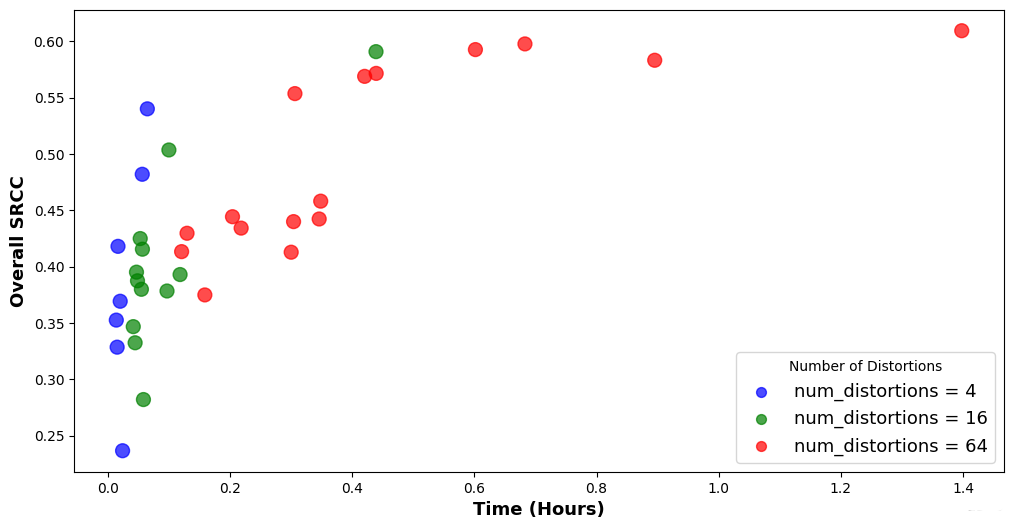
\includegraphics[keepaspectratio,width=13.5cm]{img/num_dist_cls.png}
    \caption{Overall SRCC for XGB Classifier and MLP Classifier with different numbers of distortions. Similar to \autoref{fig:NumDistReg}, this figure shows better performance with larger datasets but longer training times.}
    \label{fig:NumDistCls}
\end{figure}

\clearpage
\section{Cross-Dataset Evaluation}
\label{sec:CrossData}
The performance of the four different models, trained on SCIN\textsubscript{distorted}, F17K\textsubscript{distorted}, and COMB\textsubscript{distorted} datasets, was evaluated through cross-dataset testing. This means the models were tested on both the SCIN\textsubscript{distorted} and F17K\textsubscript{distorted} individually, as shown in \autoref{table:srcc_results}. This table helps to understand how well the models perform on different datasets and shows how well each model can adapt to different datasets, demonstrating their ability to generalize. \par 
 \begin{table}[ht]
    \centering
    \begin{tabular}{|l|c|c|}
        \hline
        \textbf{Model} & \textbf{SCIN\textsubscript{distorted}} & \textbf{F17K\textsubscript{distorted}} \\
        \hline
        COMB\textsubscript{distorted} MLP Regressor & \underline{0.66} & \underline{0.75} \\
        COMB\textsubscript{distorted} XGB Regressor & 0.65 & 0.73 \\
        COMB\textsubscript{distorted} XGB Classifier & 0.58 & 0.61 \\
        COMB\textsubscript{distorted} MLP Classifier & 0.43 & 0.46 \\
        \hline
        F17K\textsubscript{distorted} MLP Regressor & 0.54 & 0.69 \\
        SCIN\textsubscript{distorted} MLP Regressor & 0.62 & 0.49 \\
        F17K\textsubscript{distorted} XGB Regressor & 0.53 & 0.67 \\
        SCIN\textsubscript{distorted} XGB Regressor & 0.61 & 0.48 \\
        SCIN\textsubscript{distorted} MLP Classifier & 0.53 & 0.45 \\
        F17K\textsubscript{distorted} MLP Classifier & 0.47 & 0.58 \\
        SCIN\textsubscript{distorted} XGB Classifier & 0.54 & 0.43 \\
        F17K\textsubscript{distorted} XGB Classifier & 0.46 & 0.59 \\
        \hline
    \end{tabular}
    \caption{Spearman’s Rank Correlation Coefficient (SRCC) of Different Models on SCIN\textsubscript{distorted} and F17K\textsubscript{distorted} Datasets.}
    \label{table:srcc_results}
\end{table}


\section{Loss Curves}
\label{sec:LossCurveAnalysis}
The loss curve in \autoref{fig:loss} shows how the model’s loss decreases over time for each dermatology quality criterion during training. This graph helps to identify which criteria have higher or lower loss, indicating areas where the model performs well or needs improvement. \par
\vspace{\baselineskip}
\noindent
This plot shows that as training progresses, the loss for most criteria steadily decreases, indicating that the model is learning and improving. Some criteria such as background, orientation, and field of view have higher loss values, meaning the model finds these criteria more challenging, and there should be more focus on improving performance for these specific distortions. On the other hand, criteria with lower loss, like color calibration and resolution, indicate that the model performs relatively well in these areas. The training process was set to run for a maximum of 500 iterations, with early stopping enabled to avoid overfitting, which stops the training when the model’s performance does not to improve.\par
\clearpage
\begin{figure}[ht]
    \centering
    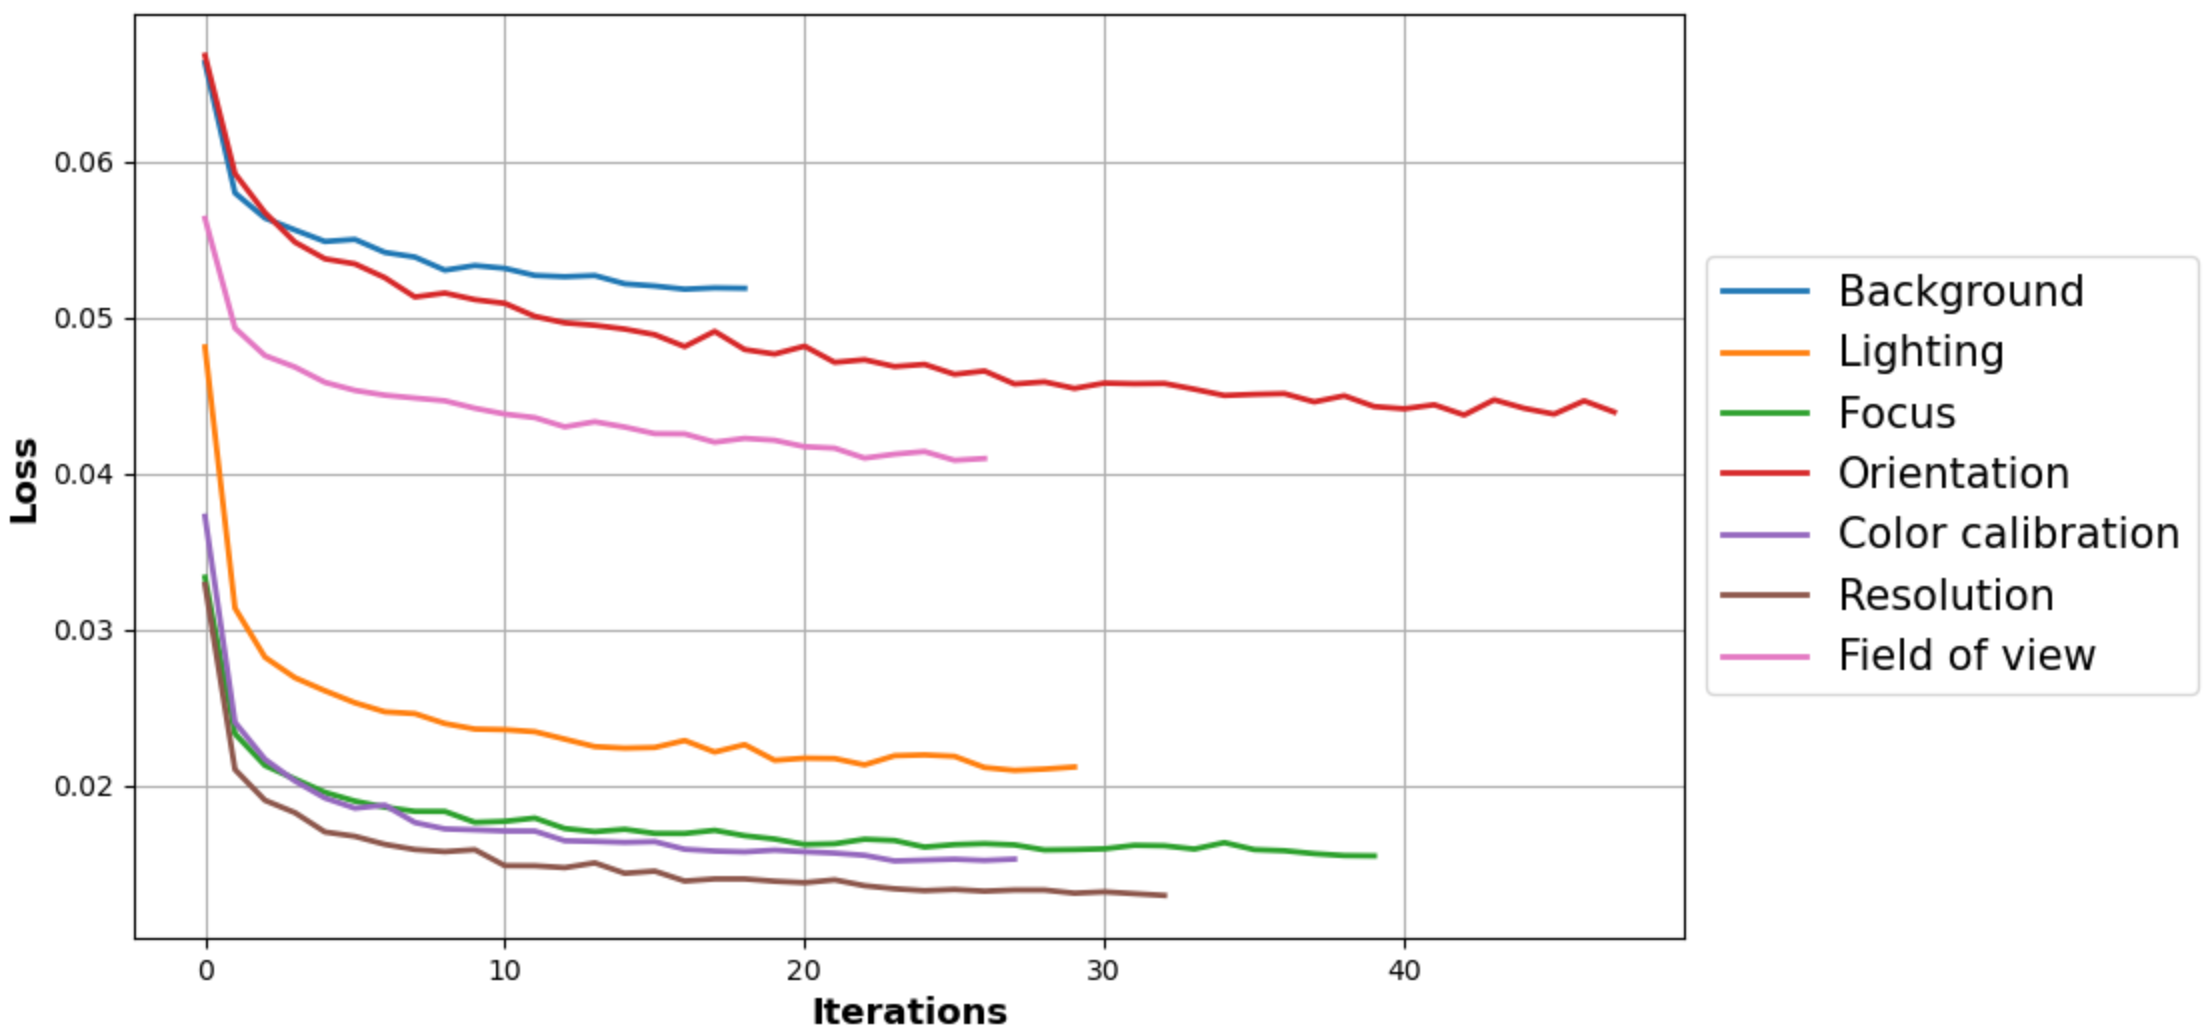
\includegraphics[keepaspectratio,width=13cm]{img/loss.png}
    \caption{ Loss curve showing the reduction in loss for each distortion criterion during the training process. Each line represents a different criterion, showing how the model’s performance improves with each iteration.}
    \label{fig:loss}
\end{figure}


\section{Parallel Coordinate Plot}
\label{sec:ParallelCoordinatePlot}
The parallel coordinate plot in \autoref{fig:ModelSRCC} compares the best-performing models across seven dermatology quality criteria, including the overall SRCC. This plot helps visualize variations in model performance for each quality criterion and the overall score, making it easier to see which models perform well in different areas. \par
\begin{figure}[ht]
    \centering
    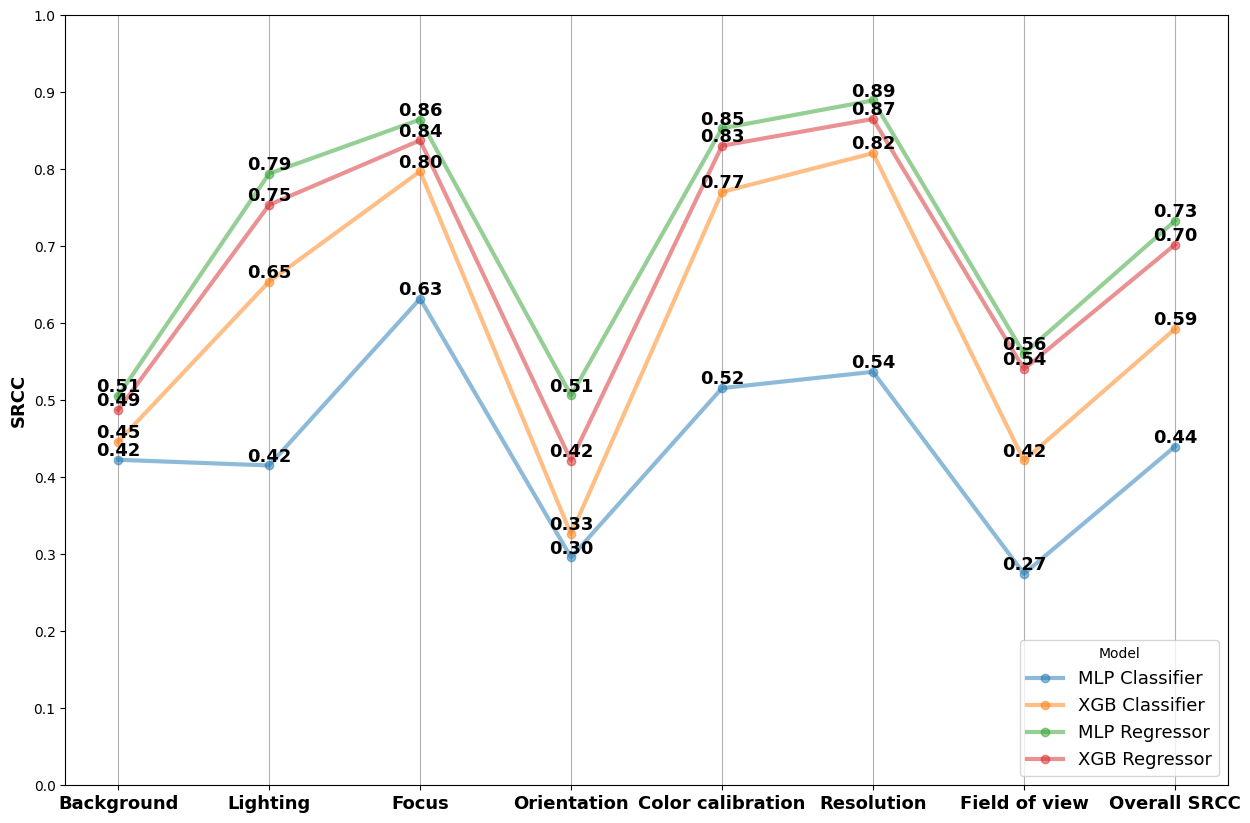
\includegraphics[keepaspectratio,width=12.5cm]{img/Model_SRCC.png}
    \caption{Parallel coordinate plot showing the best SRCC values for the four different models across the seven criteria and the overall SRCC. This plot highlights how each model performs in different areas and shows that the MLP Regressor generally performs the best.}
    \label{fig:ModelSRCC}
\end{figure}

\clearpage
\section{Confusion Matrices}
\label{sec:ConfusionMatrices}
The confusion matrices in \autoref{fig:confusion_matrices} show how well the MLP Regressor model performs on the F17K\textsubscript{distorted} dataset for each distortion criterion. These matrices help visualize where the model makes correct predictions and where it makes errors, providing a detailed view of its accuracy. Additionally, they reveal any biases the model might have towards certain severity levels, showing if it tends to predict only low or high severity levels or if its predictions are skewed in some way. \par
\vspace{\baselineskip}
\begin{figure}[ht]
    \centering
    \begin{subfigure}[b]{0.32\textwidth}
        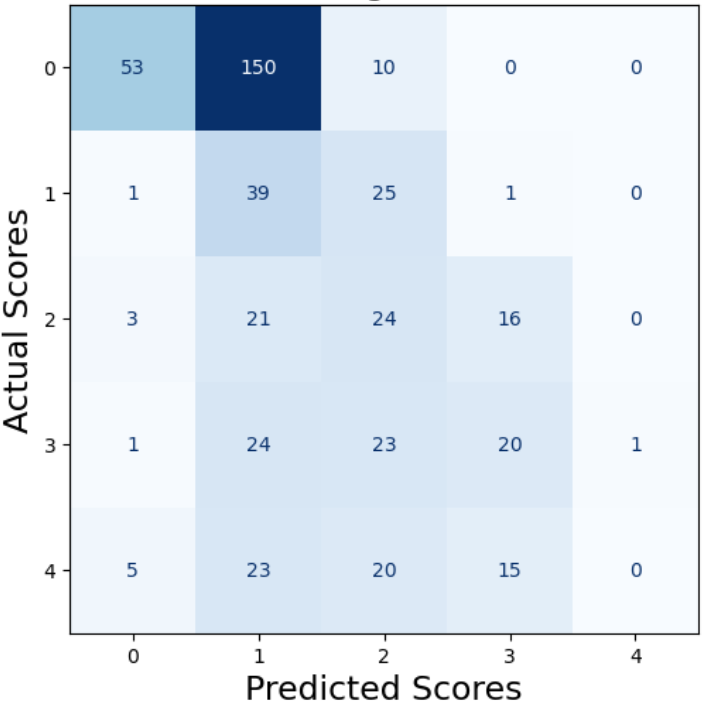
\includegraphics[width=\textwidth]{img/cm/bg.png}
        \caption{Background}
        \label{fig:cm_bg}
    \end{subfigure}
    \hfill
    \begin{subfigure}[b]{0.32\textwidth}
        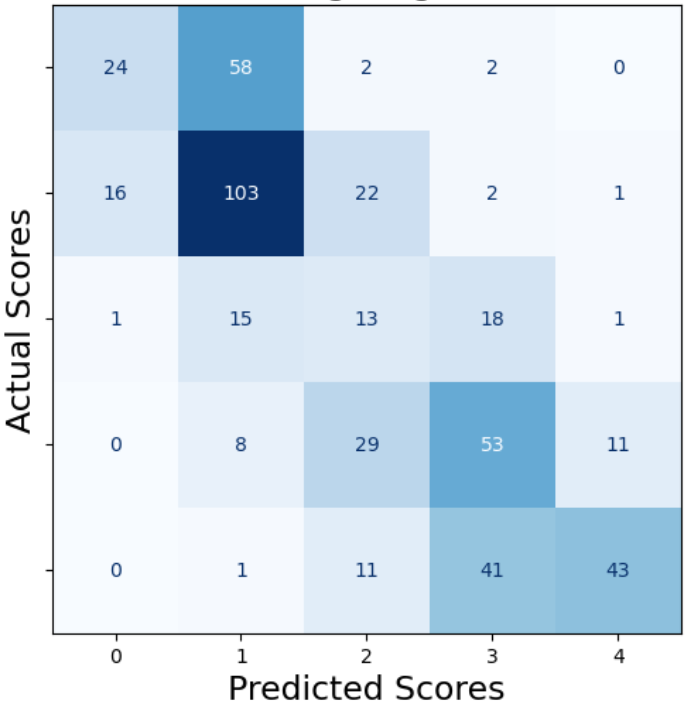
\includegraphics[width=\textwidth]{img/cm/light.png}
        \caption{Lighting}
        \label{fig:cm_light}
    \end{subfigure}
    \hfill
    \begin{subfigure}[b]{0.32\textwidth}
        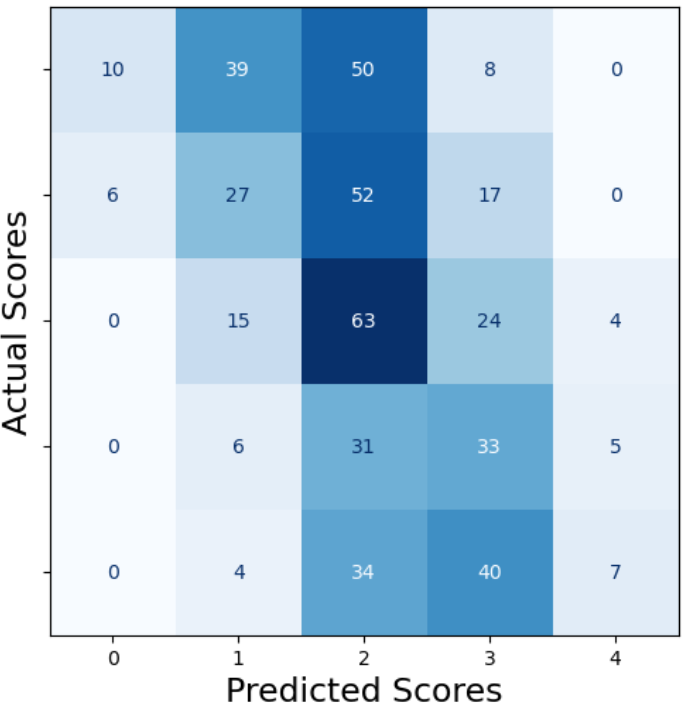
\includegraphics[width=\textwidth]{img/cm/orient.png}
        \caption{Orientation}
        \label{fig:cm_orient}
    \end{subfigure} 

    \begin{subfigure}[b]{0.24\textwidth}
        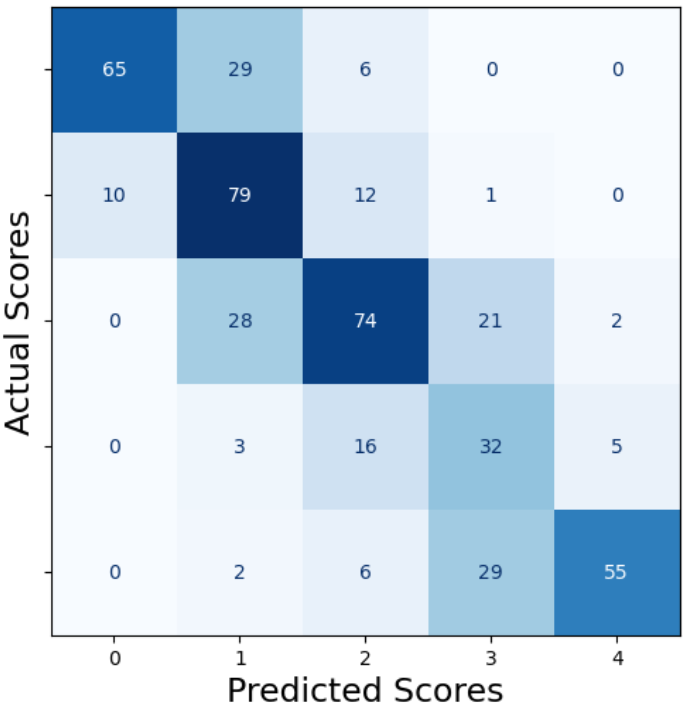
\includegraphics[width=\textwidth]{img/cm/foc.png}
        \caption{Focus}
        \label{fig:cm_foc}
    \end{subfigure}
    \hfill
    \begin{subfigure}[b]{0.24\textwidth}
        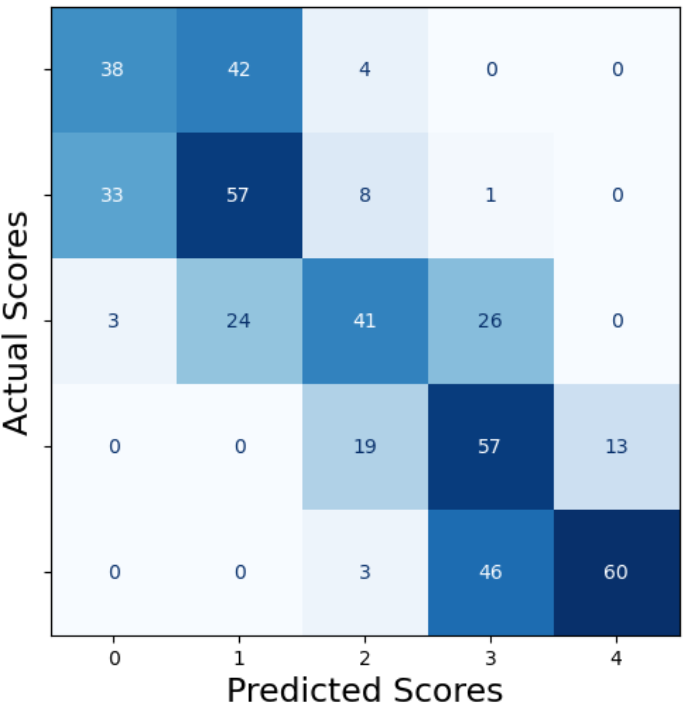
\includegraphics[width=\textwidth]{img/cm/cc.png}
        \caption{Color Calibration}
        \label{fig:cm_cc}
    \end{subfigure}
    \hfill
    \begin{subfigure}[b]{0.24\textwidth}
        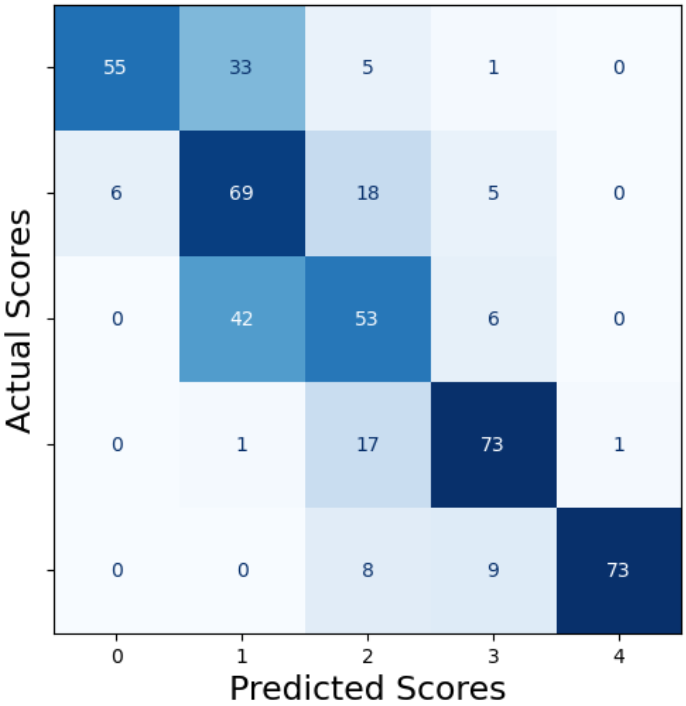
\includegraphics[width=\textwidth]{img/cm/res.png}
        \caption{Resolution}
        \label{fig:cm_res}
    \end{subfigure}
    \hfill
    \begin{subfigure}[b]{0.24\textwidth}
        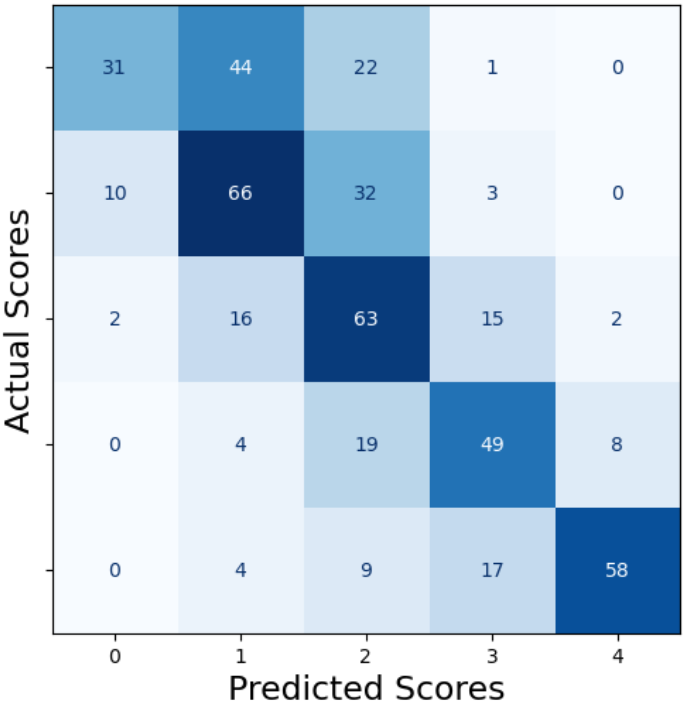
\includegraphics[width=\textwidth]{img/cm/fov.png}
        \caption{Field of View}
        \label{fig:cm_fov}
    \end{subfigure}
    \caption{Confusion matrices for the MLP Regressor model evaluated on the F17K\textsubscript{distorted} dataset. Each matrix corresponds to a specific distortion criterion and shows the actual scores on the y-axis and the predicted scores on the x-axis. Darker shades indicate higher counts, highlighting where the model's predictions match the actual values and where discrepancies occur.}
    \label{fig:confusion_matrices}
\end{figure}
\noindent
For the background criterion (\autoref{fig:cm_bg}), the model mostly predicts lower severity levels, showing a habit of underestimating the severity of background distortions. In the lighting criterion (\autoref{fig:cm_light}), the model’s predictions are quite accurate, though there are some differences across the severity levels. When it comes to orientation (\autoref{fig:cm_orient}), the model shows a tendency to predict middle severity levels for these distortions. \par
\vspace{\baselineskip}
\noindent
The focus criterion (\autoref{fig:cm_foc}) shows that the model performs well, with accurate predictions across different severity levels. For color calibration (\autoref{fig:cm_cc}, the model shows good performance with some differences but no significant bias. In the resolution criterion (\autoref{fig:cm_res}), the model’s predictions are quite accurate across different severity levels. Finally, for the field of view criterion (\autoref{fig:cm_fov}), the model performs well, with predictions spread across severity levels without significant bias. \par

\clearpage
\section{Performance Metrics}
\label{sec:PerformanceMetrics}
The performance metrics of the final MLP regressor model on individual dermatology quality criteria are shown in \autoref{table:performance_metrics}. This table provides a detailed view of how well the model performs across different criteria and overall. It includes four key metrics: Mean Absolute Error (MAE), R\textsuperscript{2}, Spearman Rank Correlation Coefficient (SRCC), and Cohen’s Kappa. \par
\vspace{\baselineskip}
\noindent
This table shows the model’s strengths and weaknesses. For example, the SRCC values for background, orientation, and field of view are the lowest among the seven criteria, indicating that the model struggles more with these distortions. On the other hand, higher SRCC values for criteria like lighting and focus suggest better model performance in those areas. \par
 \begin{table}[ht]
    \centering
    \begin{tabular}{|l|c|c|c|c|}
        \hline
        \textbf{Criteria} & \textbf{MAE} & \textbf{R\textsuperscript{2}} & \textbf{SRCC} & \textbf{Cohen's Kappa} \\
        \hline
        Background & 0.9684 & 0.2595 & 0.5422 & 0.4399 \\
        Lighting & 0.5726 & 0.6440 & 0.8028 & 0.7913 \\
        Focus & 0.4042 & 0.7385 & 0.8622 & 0.8568 \\
        Orientation & 0.9895 & 0.1824 & 0.4735 & 0.4102 \\
        Color calibration & 0.4905 & 0.7334 & 0.8622 & 0.8583 \\
        Resolution & 0.3642 & 0.7656 & 0.8722 & 0.8726 \\
        Field of view & 0.5474 & 0.5976 & 0.7710 & 0.7660 \\
        \hline
        \textbf{Overall} & \textbf{0.6195} & \textbf{0.5646} & \textbf{0.7507} & \textbf{0.7396} \\
        \hline
    \end{tabular}
    \caption{Performance Metrics for Each Distortion Criteria}
    \label{table:performance_metrics}
\end{table}

\section{Model Predictions}
\label{sec:VisualizingPredictions}
To understand how well the model performs on the two test sets (SCIN\textsubscript{synthetic} and SCIN\textsubscript{authentic}), radar charts were used. These charts show the different criteria around the outside, with the severity levels ranging from the center (0) to the outer edge (1), indicating high distortion for each criterion. These visualizations give a clear and simple view of the model’s performance, showing both its strengths and areas where it can improve. \par
\subsection{Visualizations for Synthetic Distorted Images}
\label{subsec:SyntheticDistortedImages}
\autoref{fig:synthetic} shows how the model predicts distortions for synthetic test images. These visualizations compare the model’s predictions with the actual distortions. This layout also helps to see how accurately the model can predict different types of distortions.\par
\vspace{\baselineskip}
\noindent
The first column shows the original image, the second shows the distorted image, the third contains the actual labels, and the fourth presents the model’s predictions. \par
\begin{figure}[ht]
    \centering
    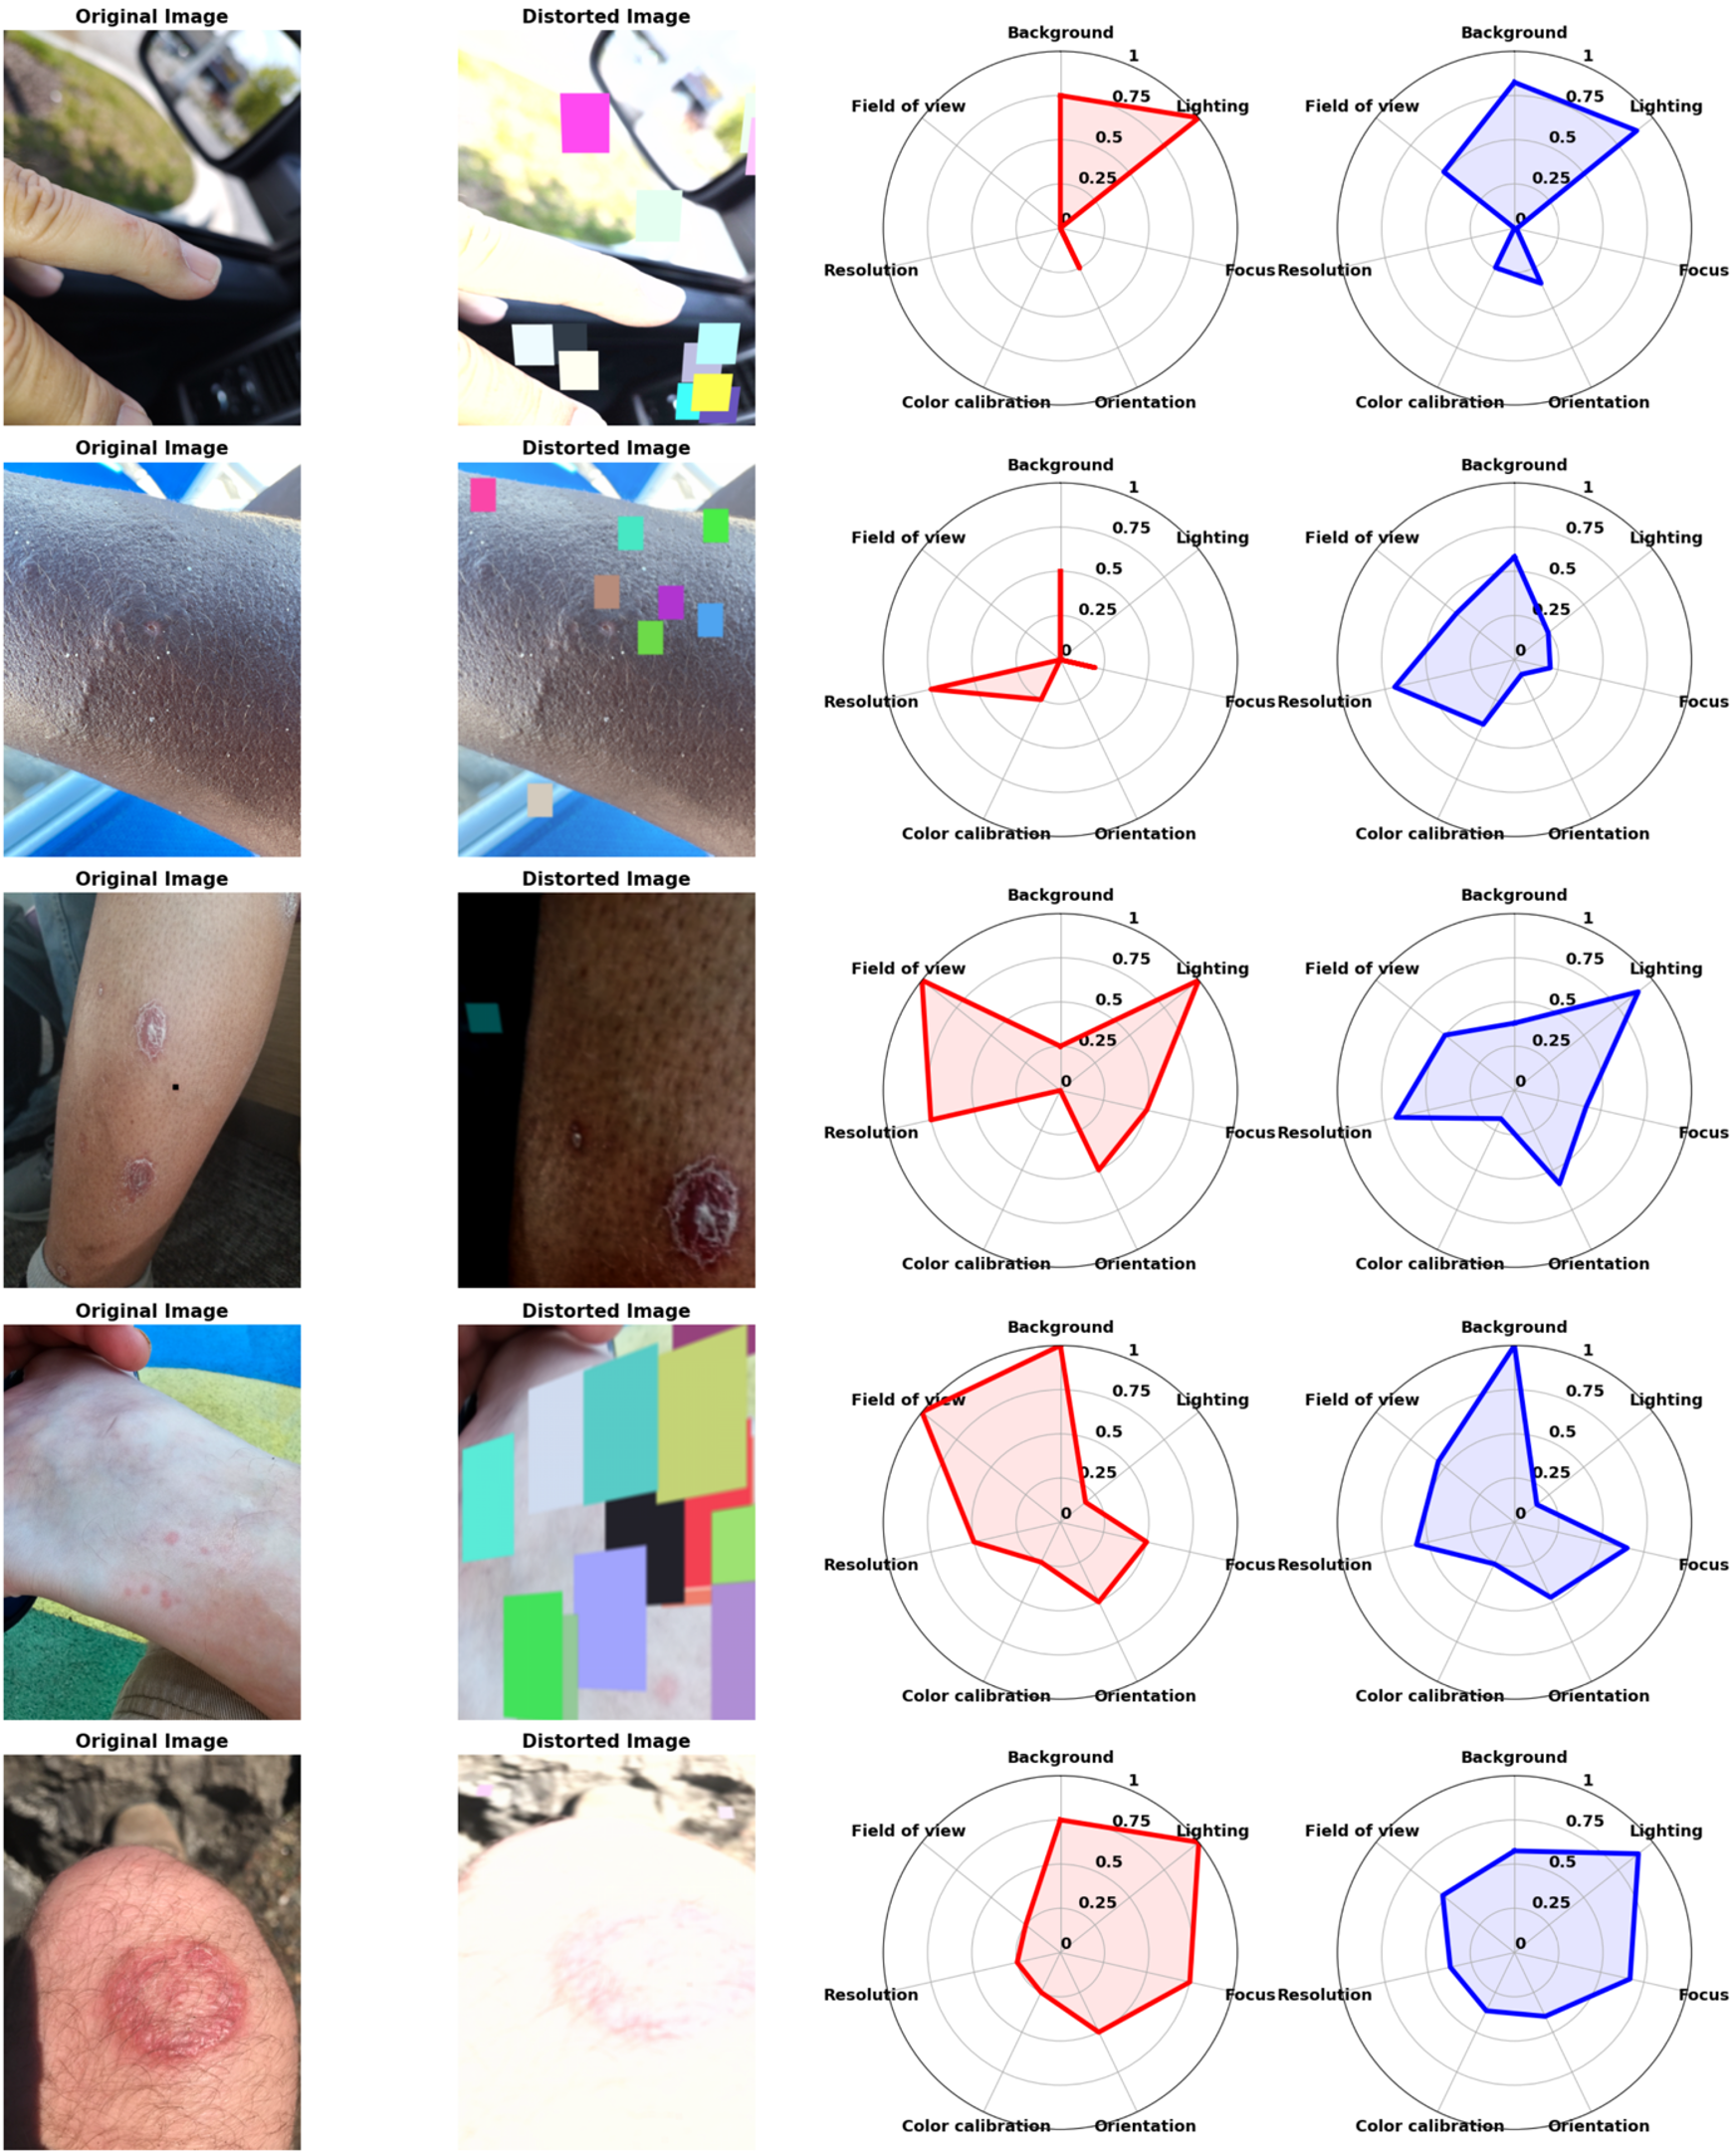
\includegraphics[keepaspectratio,width=15cm]{img/synthetic.png}
    \caption{Comparison of model predictions with synthetic distorted test images using a four-column layout. The four-column layout shows the original image, the distorted image, the actual labels, and the model's predictions.}
    \label{fig:synthetic}
\end{figure}

\subsection{Visualizations for Authentic Images}
\label{subsec:AuthenticImages}
\autoref{fig:authentic} shows the model’s performance on authentic images, comparing its predictions with human-labeled scores. This helps to understand how well the model works in real-world situations and  how closely the model’s predictions match with human evaluations. \par
\vspace{\baselineskip}
\noindent
The first column shows the image, the second column displays the human-labeled scores, and the third column presents the model’s predictions. \par
\begin{figure}[ht]
    \centering
    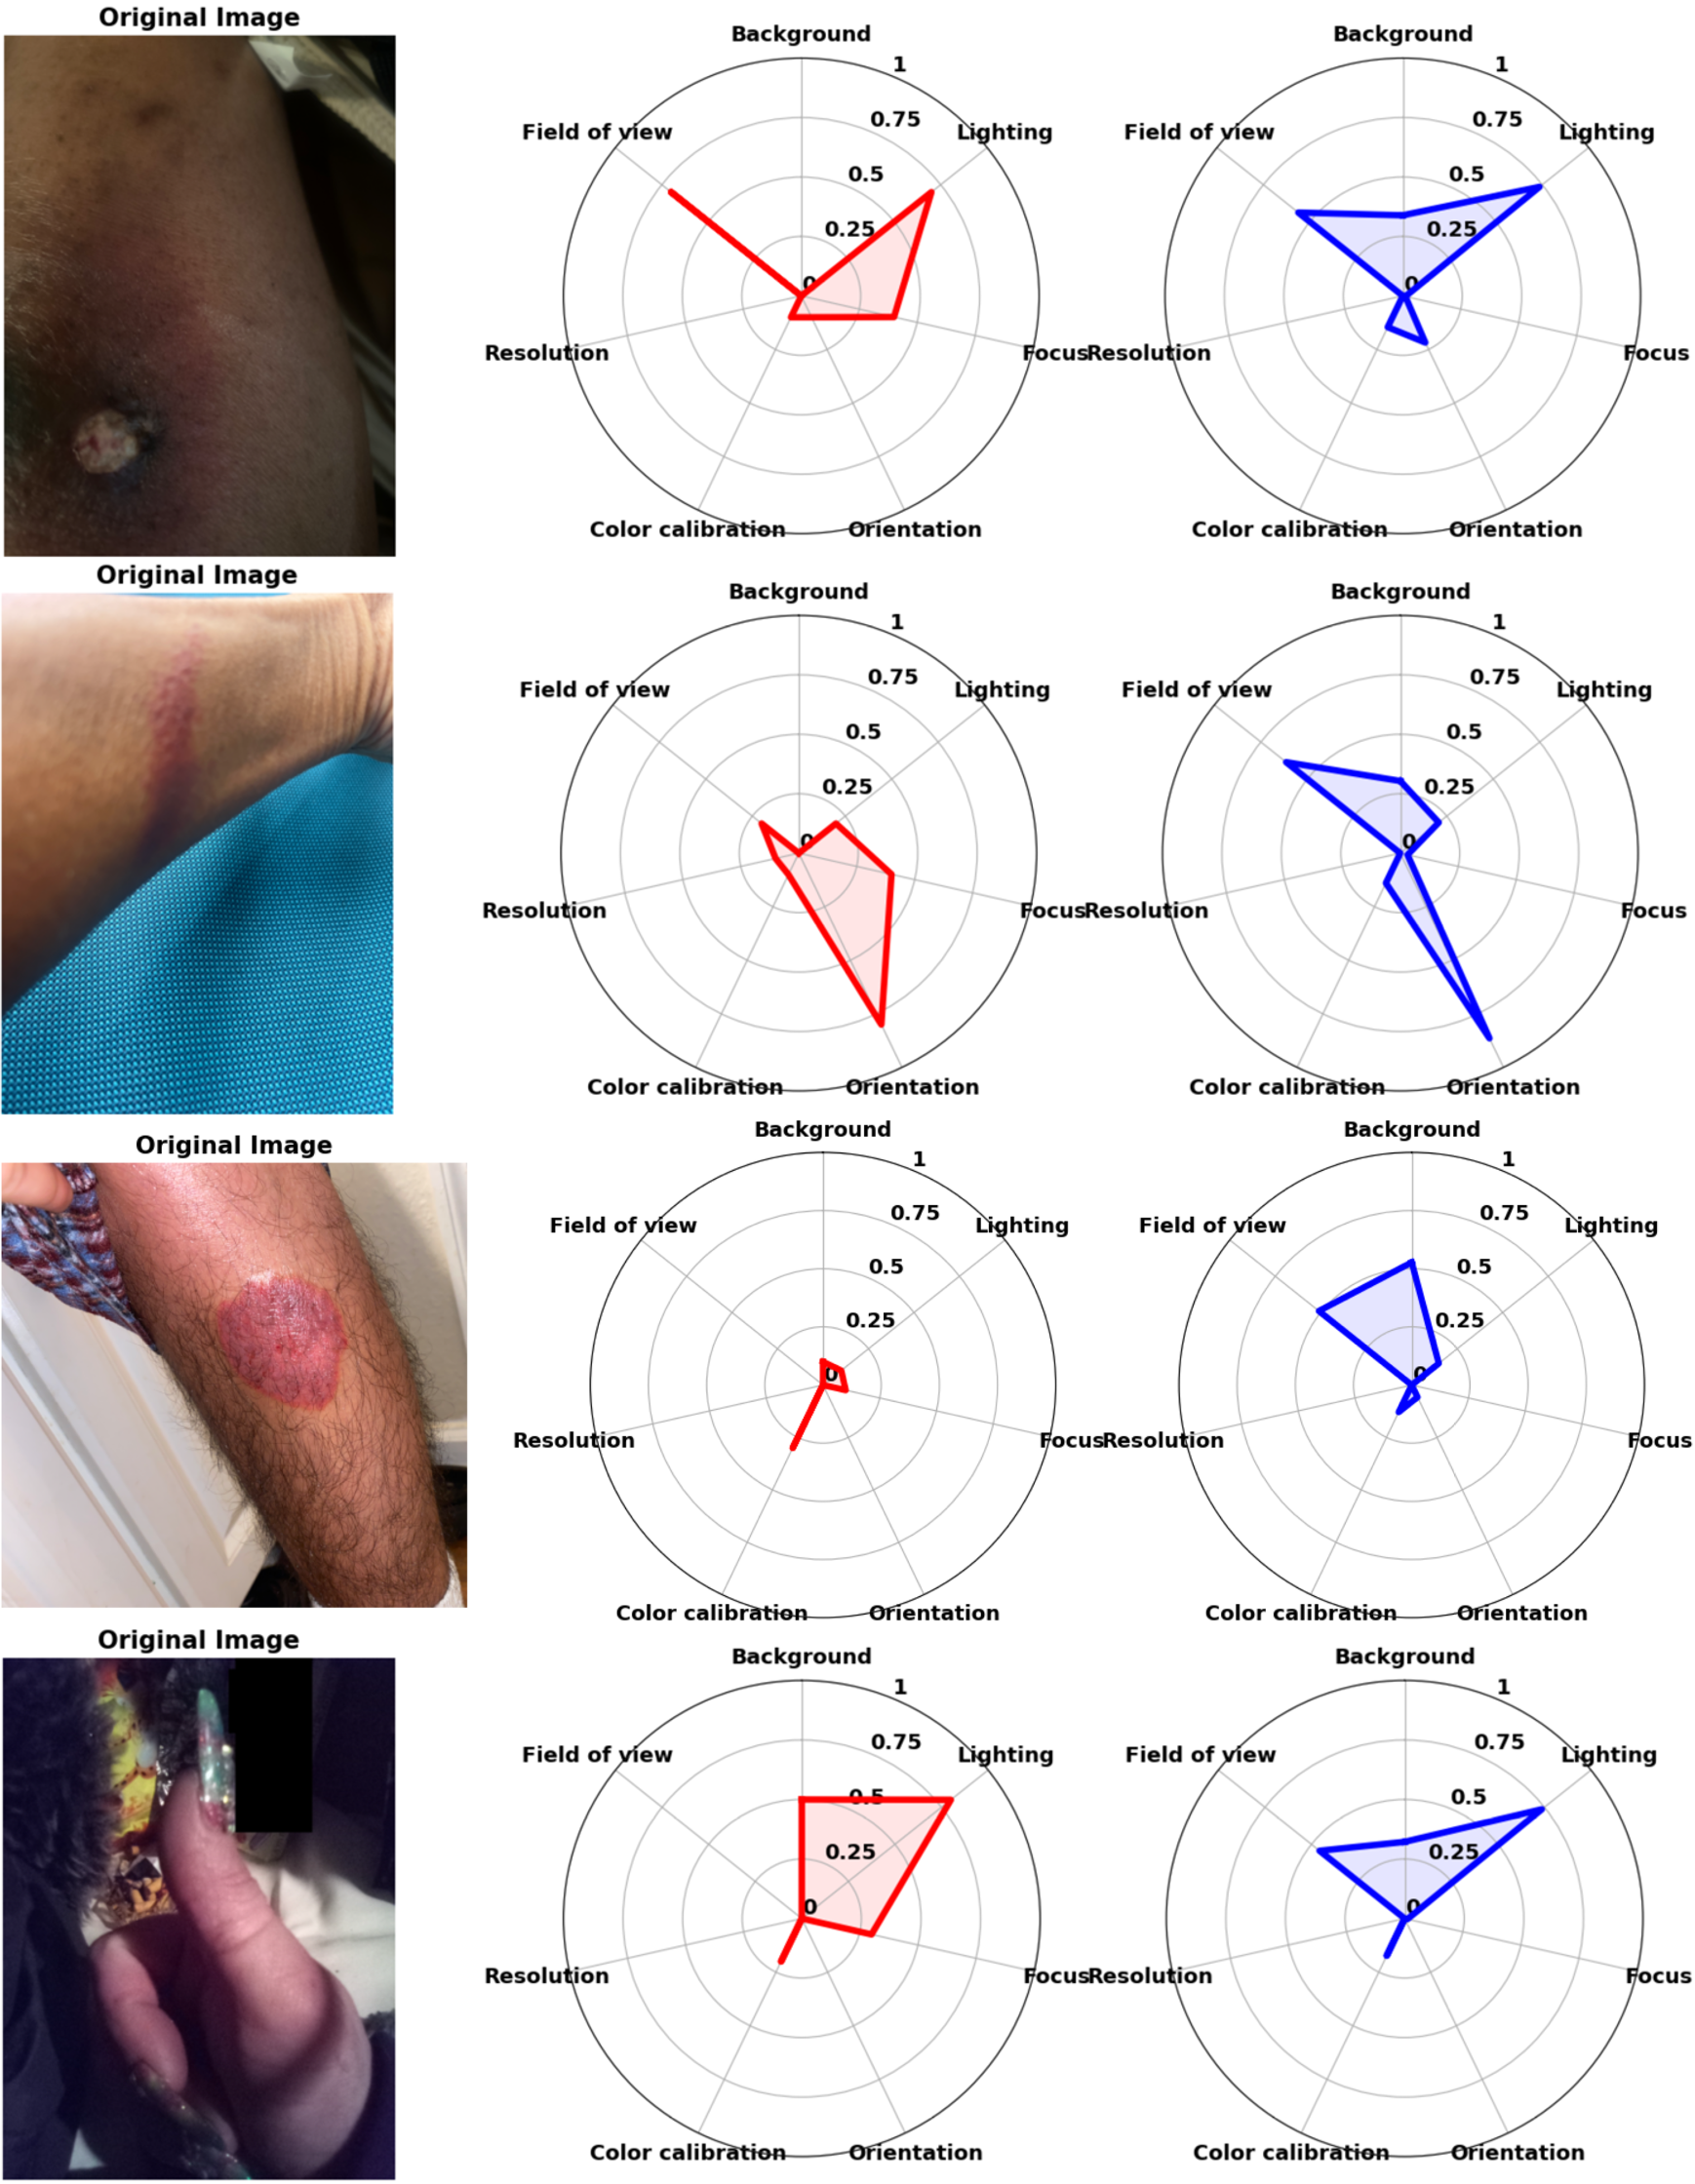
\includegraphics[keepaspectratio,width=15cm]{img/authentic.png}
    \caption{Comparison of model predictions with human-labeled scores for authentic images using a three-column layout. The three-column layout shows the image, the human-labeled scores, and the model's predictions.}
    \label{fig:authentic}
\end{figure}


\clearpage
\section{Assessing Training and Testing Images Quality}
\label{sec:TestingFilteredImages}
To verify the quality of the images used for training and see how they change after synthetic distortion, radar charts were created. These charts show the quality of the original training images and how they are affected by the distortions. Additionally, the quality of both the synthetic and authentic test images is assessed using the same method. These radar charts show a simple visual representation of the quality and the level of distortion across the seven criteria. In these radar charts, the median value is shown as the blue line, while the dotted line represents the maximum value. \par
\subsection{Training Images Quality}
\label{subsec:TrainingImagesQuality}
\autoref{fig:SF} and \autoref{fig:FF} show the quality of the original SCIN\autocite{SCIN} and Fitzpatrick17k\autocite{F17K} images, and the filtered good quality images, respectively. \autoref{fig:CF} shows the quality of the combined SCIN\textsubscript{good} and F17K\textsubscript{good} images and the synthetically distorted COMB\textsubscript{distorted} images used for training the model. These charts show the differences in quality before and after filtering and distortion.\par
\vspace{\baselineskip}

\begin{figure}[ht]
    \centering
    \begin{subfigure}[b]{0.45\textwidth}
        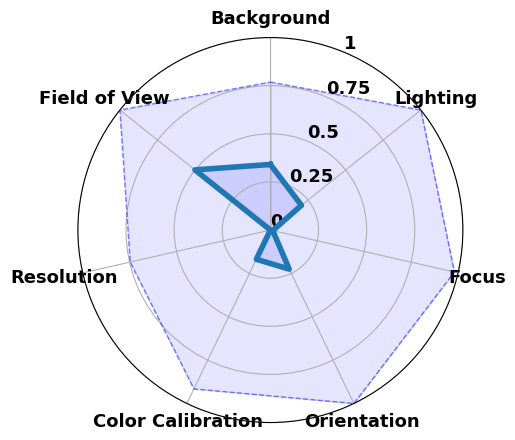
\includegraphics[width=\textwidth]{img/hept/SCIN10k.png}
        \caption{SCIN Images}
        \label{fig:SCIN10k}
    \end{subfigure}
    \hfill
    \begin{subfigure}[b]{0.45\textwidth}
        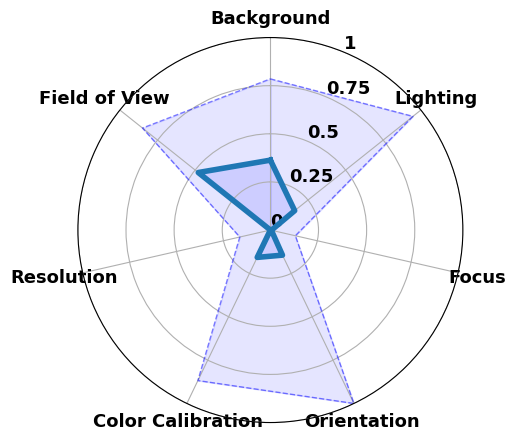
\includegraphics[width=\textwidth]{img/hept/SCIN.png}
        \caption{Filtered SCIN Images}
        \label{fig:SCIN}
    \end{subfigure}
    \hfill
    \caption{Radar charts for the SCIN dataset. (a) Original images from the SCIN dataset (10'379 images). (b) Filtered good quality images (SCIN\textsubscript{good}). Note: The blue line represents the median, and the dotted line represents the maximum.}
    \label{fig:SF}
\end{figure}
\clearpage
\vspace{\baselineskip}

\begin{figure}[ht]
    \centering
    \begin{subfigure}[b]{0.45\textwidth}
        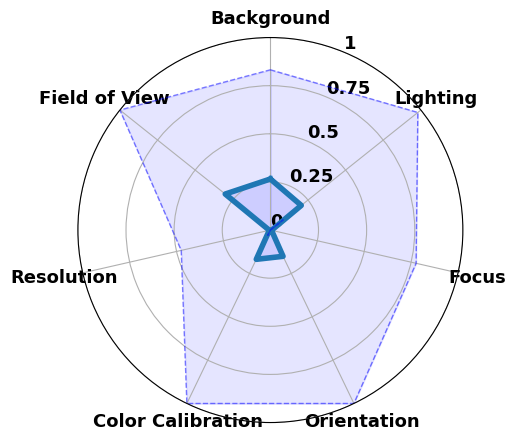
\includegraphics[width=\textwidth]{img/hept/Fitzpatrick17k.png}
        \caption{Fitzpatrick Images}
        \label{fig:Fitzpatrick17K}
    \end{subfigure}
    \hfill
    \begin{subfigure}[b]{0.45\textwidth}
        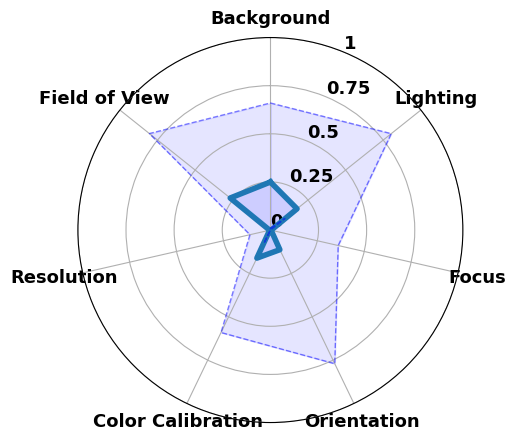
\includegraphics[width=\textwidth]{img/hept/F17K.png}
        \caption{Filtered Fitzpatrick Images}
        \label{fig:F17K}
    \end{subfigure}
    \hfill
    \caption{Radar charts for the Fitzpatrick dataset. (a) Original images from the Fitzpatrick dataset (16'577 images). (b) Filtered good quality images (F17K\textsubscript{good}). Note: The blue line represents the median, and the dotted line represents the maximum.}
    \label{fig:FF}
\end{figure}
\vspace{\baselineskip}

\begin{figure}[ht]
    \centering
    \begin{subfigure}[b]{0.45\textwidth}
        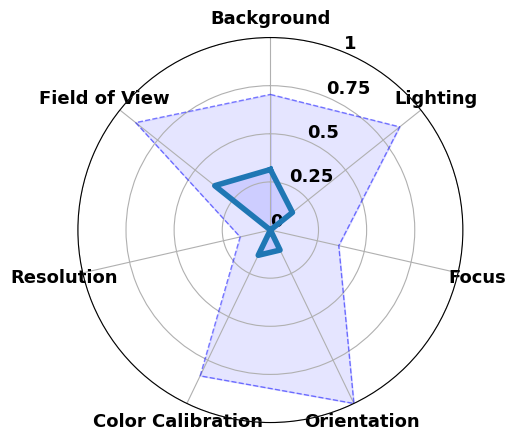
\includegraphics[width=\textwidth]{img/hept/combined.png}
        \caption{Combined SCIN and Fitzpatrick Images}
        \label{fig:combined}
    \end{subfigure}
    \hfill
    \begin{subfigure}[b]{0.45\textwidth}
        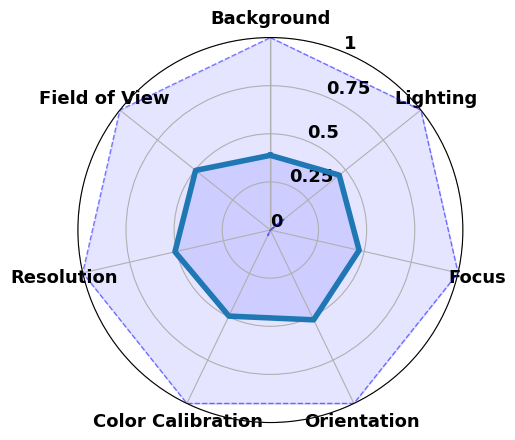
\includegraphics[width=\textwidth]{img/hept/comb_synthetic.png}
        \caption{Synthetically Distorted Images}
        \label{fig:comb_synthetic}
    \end{subfigure}
    \hfill
    \caption{Combined dataset analysis. (a) Combined SCIN\textsubscript{good} and F17K\textsubscript{good} images. (b) Synthetically distorted images (COMB\textsubscript{distorted}). Note: The blue line represents the median, and the dotted line represents the maximum.}
    \label{fig:CF}
\end{figure}

\clearpage
\subsection{Test Images Quality}
\label{subsec:TestImagesQuality}
\autoref{fig:T1} shows the quality of the SCIN\textsubscript{good} test images and the synthetically distorted SCIN\textsubscript{synthetic} test images. \autoref{fig:T2} shows the quality of the SCIN\textsubscript{authentic} test images from the SCIN dataset. These radar charts show a simple visual representation of the quality of the test images and the level of distortion across the seven criteria. \par
\vspace{\baselineskip}
\begin{figure}[ht]
    \centering
    \begin{subfigure}[b]{0.45\textwidth}
        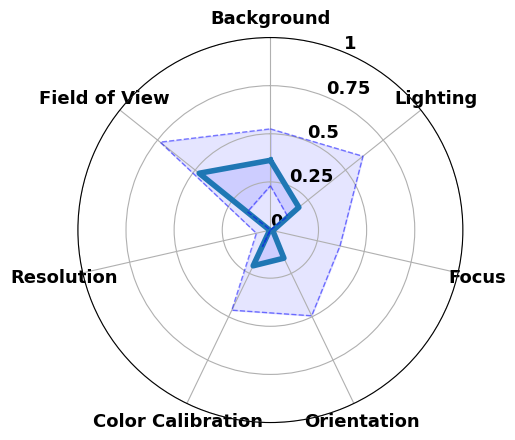
\includegraphics[width=\textwidth]{img/hept/test_70.png}
        \caption{Filtered Test Images}
        \label{fig:test_70}
    \end{subfigure}
    \hfill
    \begin{subfigure}[b]{0.45\textwidth}
        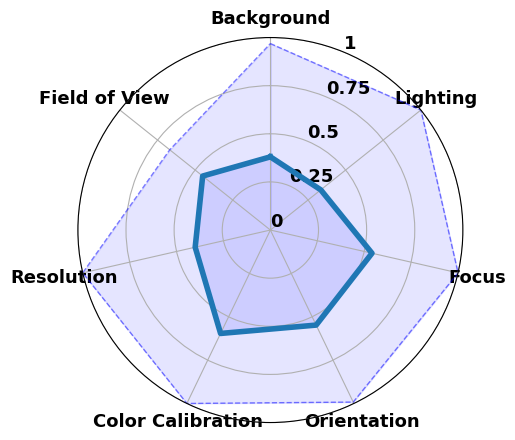
\includegraphics[width=\textwidth]{img/hept/test_70_synthetic.png}
        \caption{Synthetically Distorted Test Images}
        \label{fig:test_70_synthetic}
    \end{subfigure}
    \hfill
    \caption{Synthetic test set analysis. (a) Filtered good quality test images (70 images, independent of training set). (b) Synthetically distorted test images (SCIN\textsubscript{synthetic}) Note: The blue line represents the median, and the dotted line represents the maximum..}
    \label{fig:T1}
\end{figure}
\vspace{\baselineskip}
\begin{figure}[ht]
    \centering
    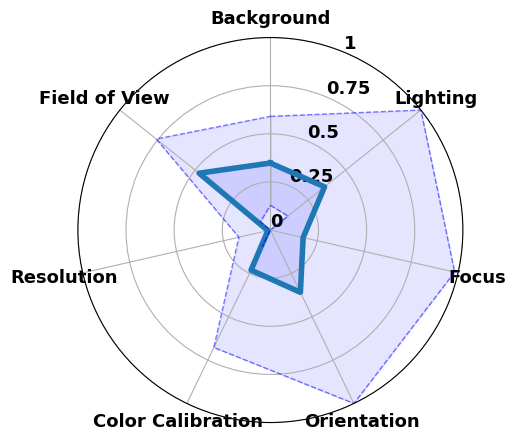
\includegraphics[keepaspectratio,width=7cm]{img/hept/test_200.png}
    \caption{Authentic test set from the SCIN dataset, independent of the training images, showing real-world distortions (SCIN\textsubscript{authentic}). Note: The blue line represents the median, and the dotted line represents the maximum.}
    \label{fig:T2}
\end{figure}

\clearpage
\section{Baseline Comparison on Synthetic and Authentic Distortions}
\label{sec:ComparisonARNIQA}
\autoref{fig:BS} compares single quality scores for synthetic distortions across different methods and \autoref{fig:BA} compares single quality scores for authentic distortions. The x-axis shows the number of images, while the y-axis shows the quality score for each image. The SRCC values in the legend tell us how well each method matches the actual scores and the main focus is on which smoothed line best matches the trend of the actual scores. \par

\begin{figure}[ht]
    \centering
    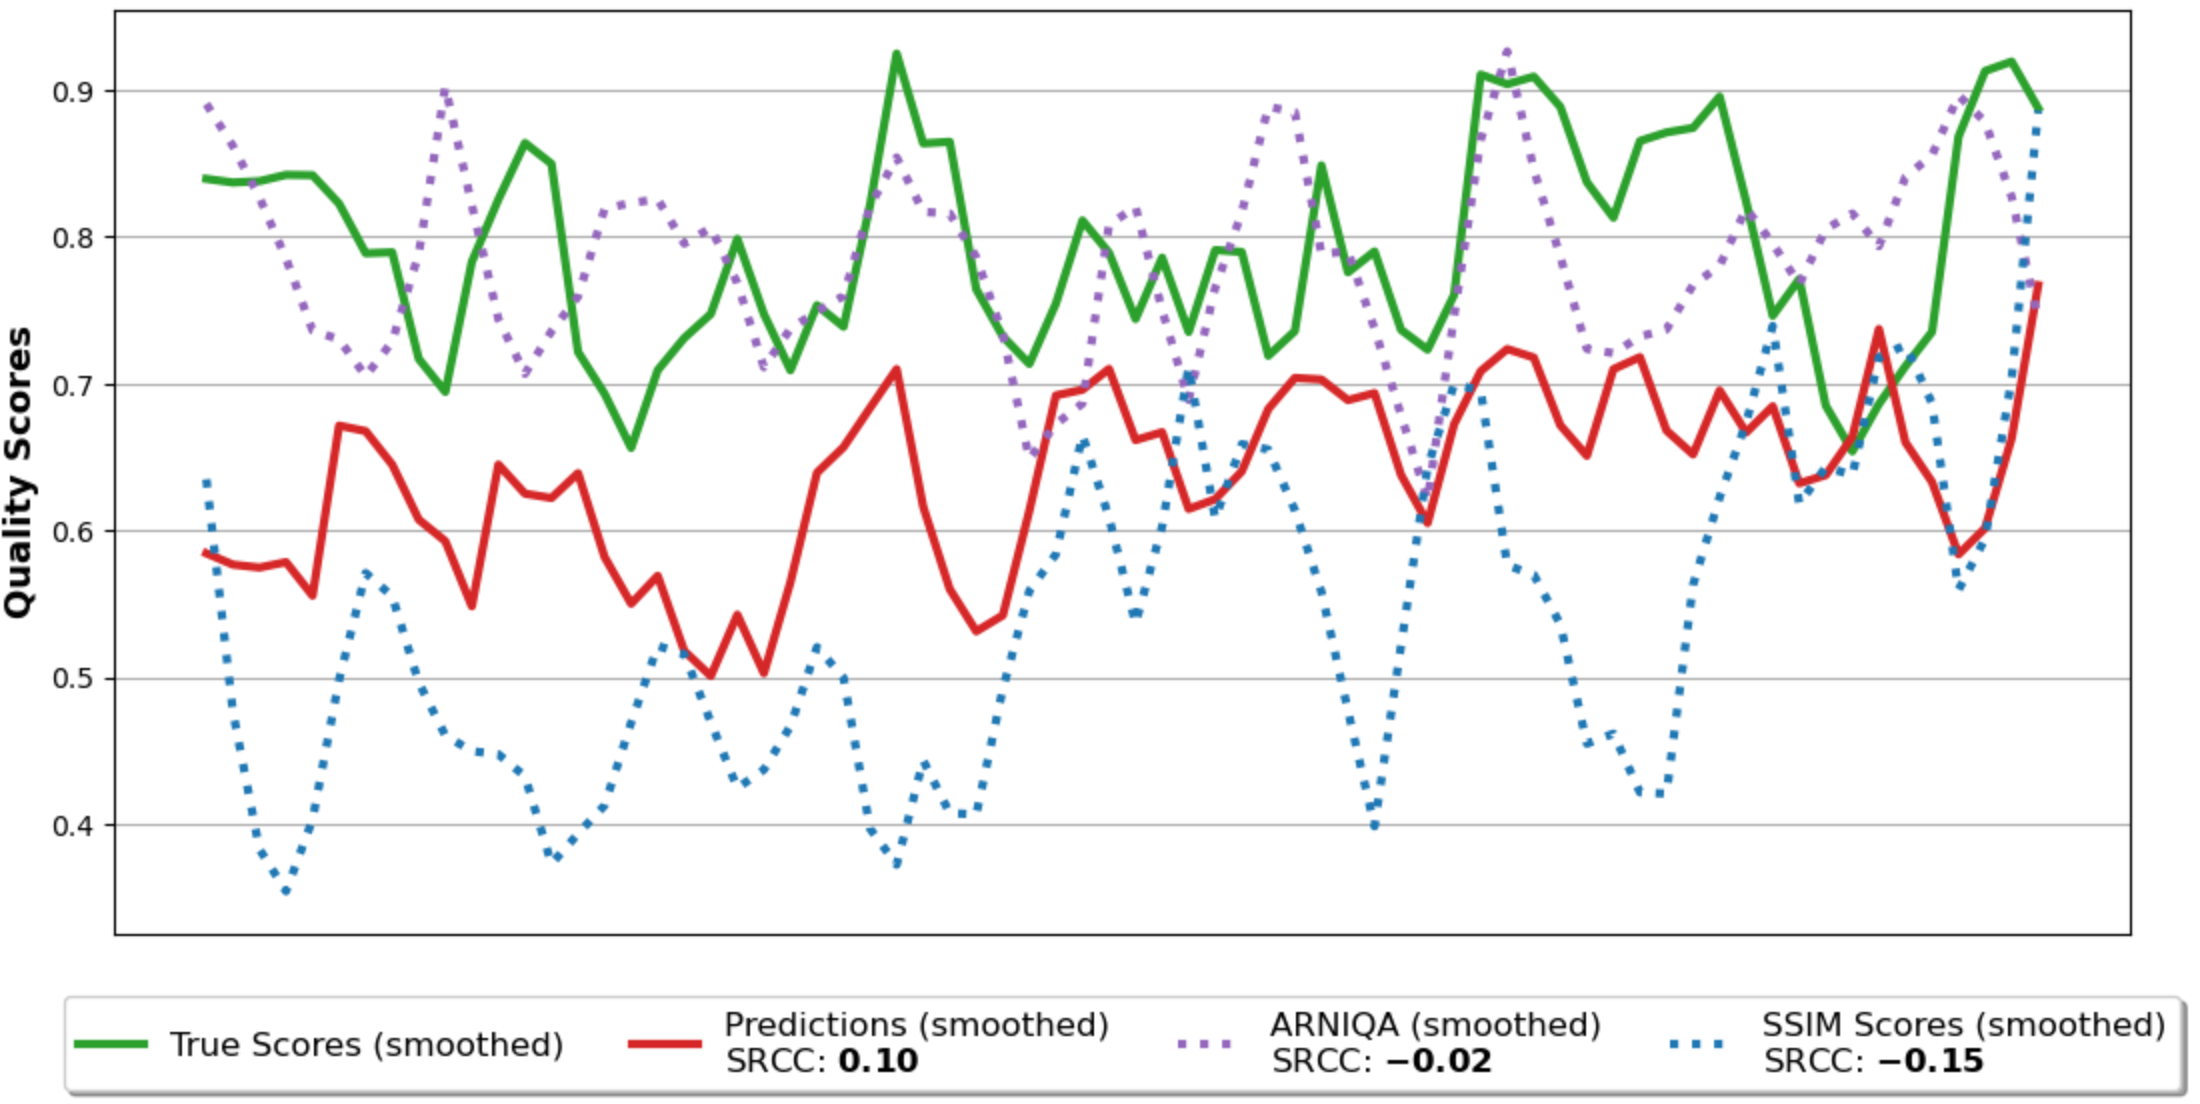
\includegraphics[keepaspectratio,width=15cm]{img/baseline_s.png}
    \caption{Comparing single quality scores for synthetic distortions using the proposed model, SSIM, and ARNIQA.}
    \label{fig:BS}
\end{figure}

\begin{figure}[ht]
    \centering
    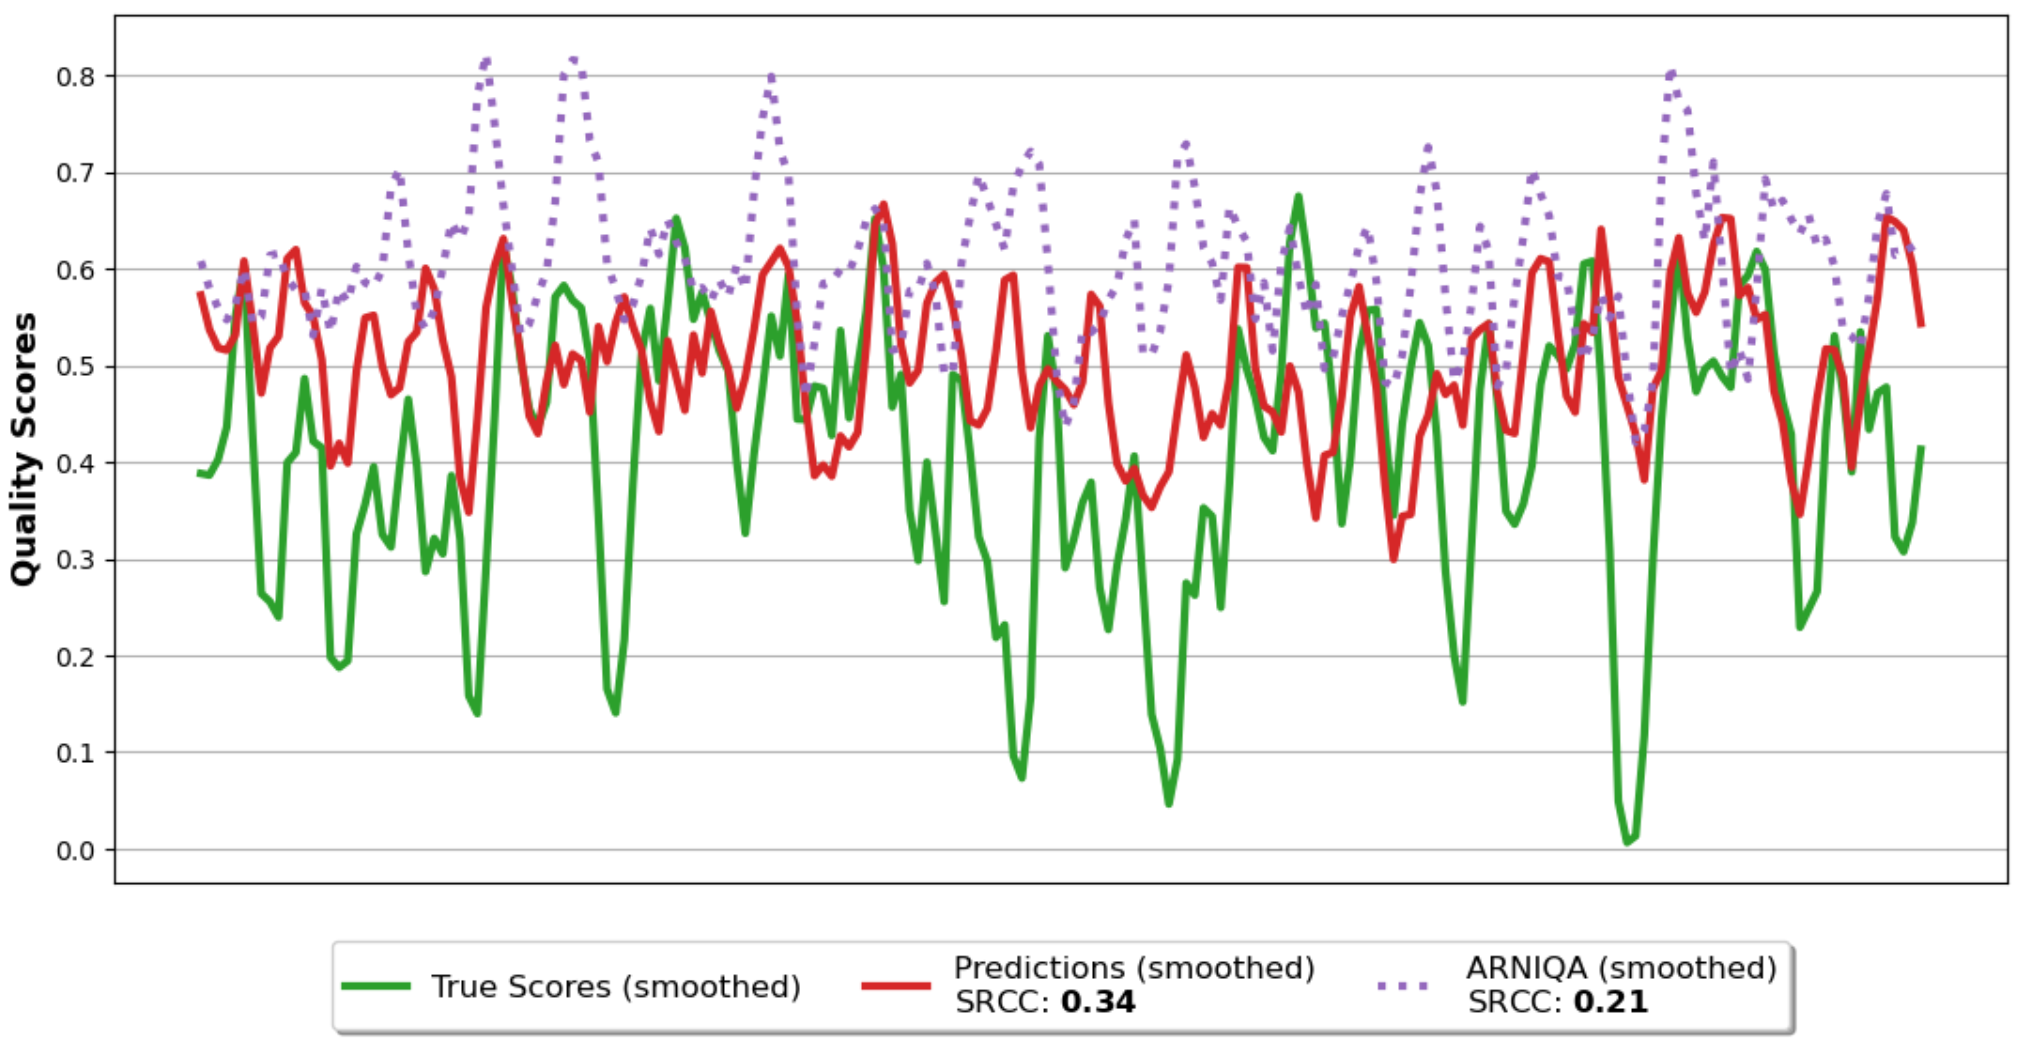
\includegraphics[keepaspectratio,width=15cm]{img/baseline_a.png}
    \caption{Comparing single quality scores for authentic distortions using the proposed model and ARNIQA.}
    \label{fig:BA}
\end{figure}

\clearpage
\subsection{Out of Distribution Testing}
\label{BO}
\autoref{fig:ood1} shows images which are different form teledermatology images. The left side shows the images, and the right side shows radar charts that indicate the model’s assessment of the seven quality criteria for each image. \par
\vspace{\baselineskip}
\begin{figure}[ht]
    \centering
    \begin{subfigure}[b]{0.48\textwidth}
        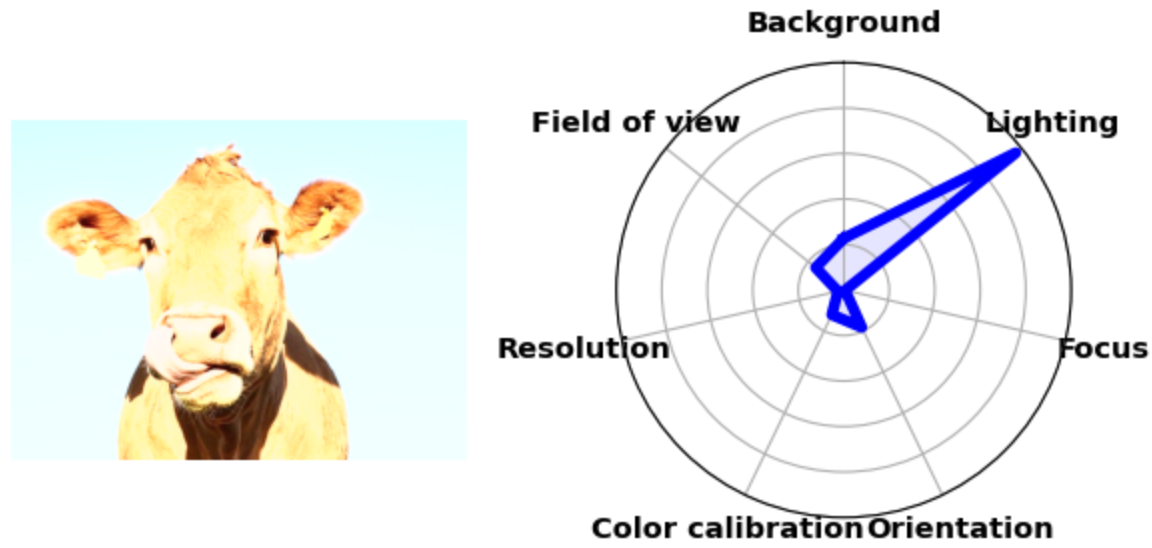
\includegraphics[width=\textwidth]{img/ood/1l.png}
        \caption{Lighting}
        \label{fig:1l}
    \end{subfigure}
    \hfill
    \begin{subfigure}[b]{0.48\textwidth}
        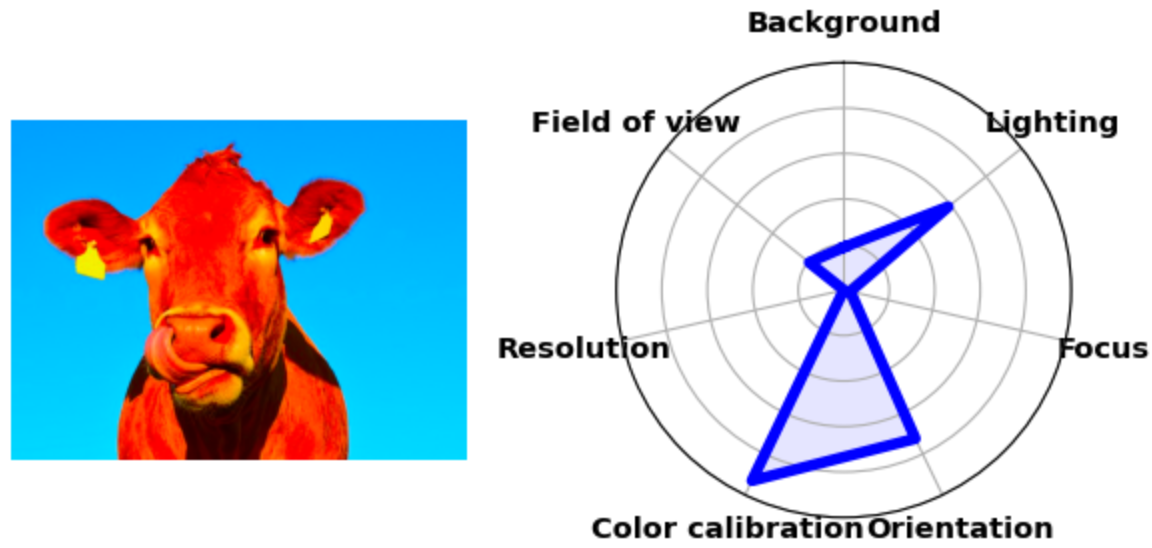
\includegraphics[width=\textwidth]{img/ood/1c.png}
        \caption{Color Calibration}
        \label{fig:1c}
    \end{subfigure}

    \begin{subfigure}[b]{0.48\textwidth}
        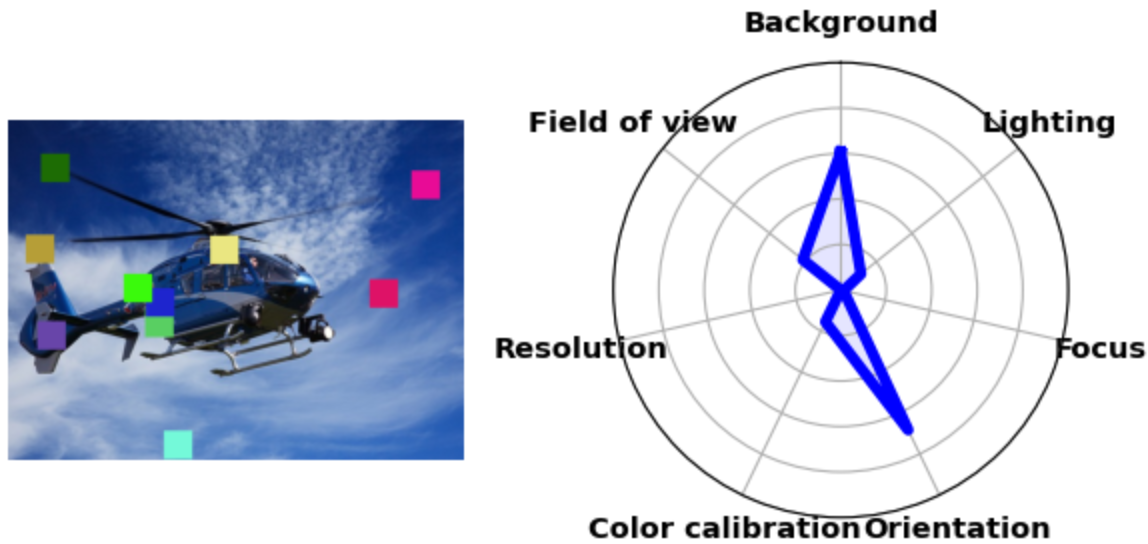
\includegraphics[width=\textwidth]{img/ood/2b.png}
        \caption{Background}
        \label{fig:2b}
    \end{subfigure}
    \hfill
    \begin{subfigure}[b]{0.48\textwidth}
        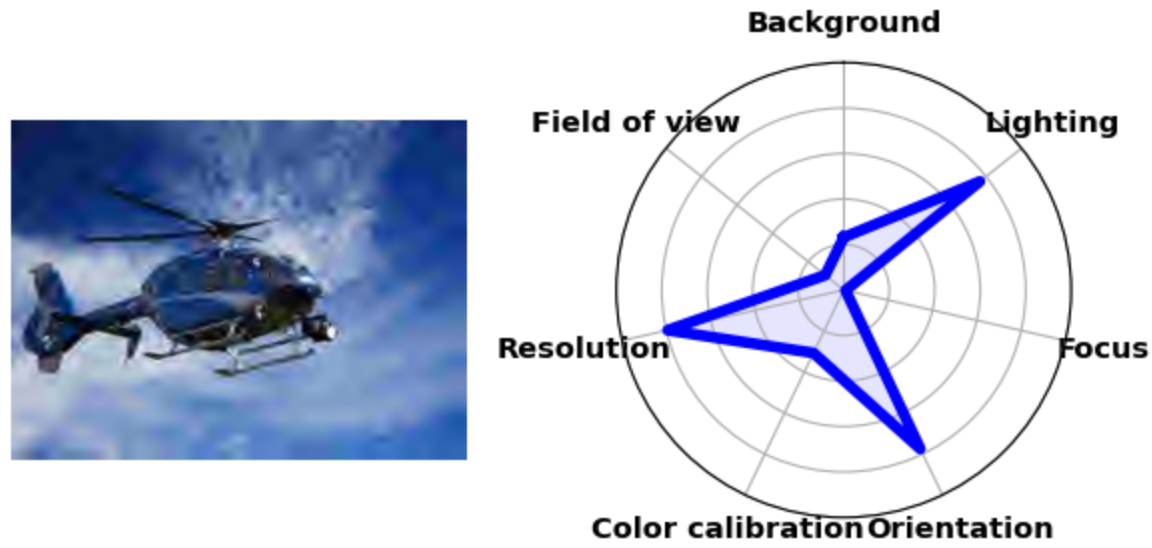
\includegraphics[width=\textwidth]{img/ood/2r.png}
        \caption{Resolution}
        \label{fig:2r}
    \end{subfigure}

    \begin{subfigure}[b]{0.48\textwidth}
        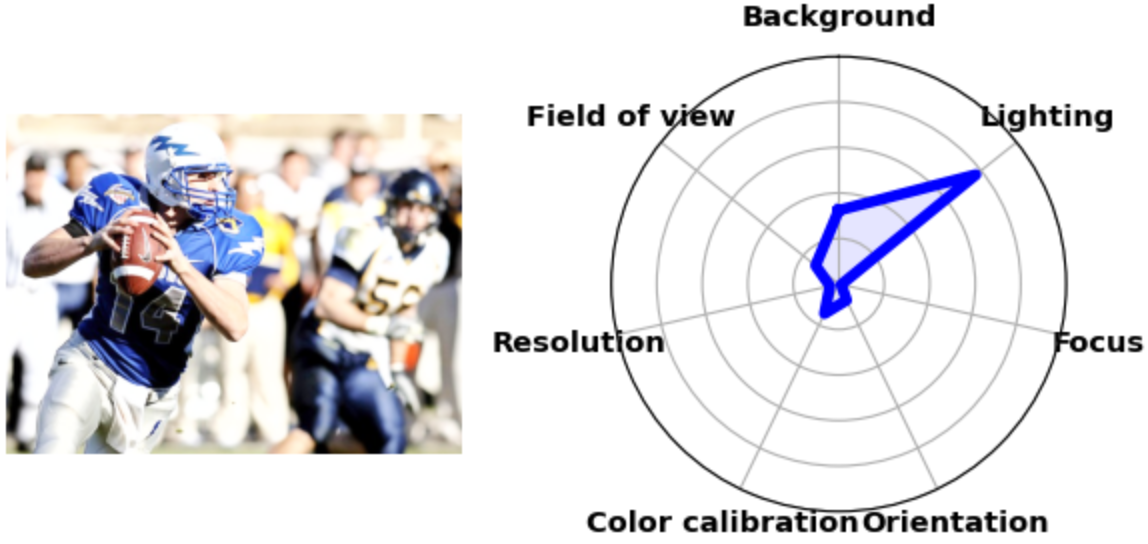
\includegraphics[width=\textwidth]{img/ood/4l.png}
        \caption{Lighting (Brighten)}
        \label{fig:4l}
    \end{subfigure}
    \hfill
    \begin{subfigure}[b]{0.48\textwidth}
        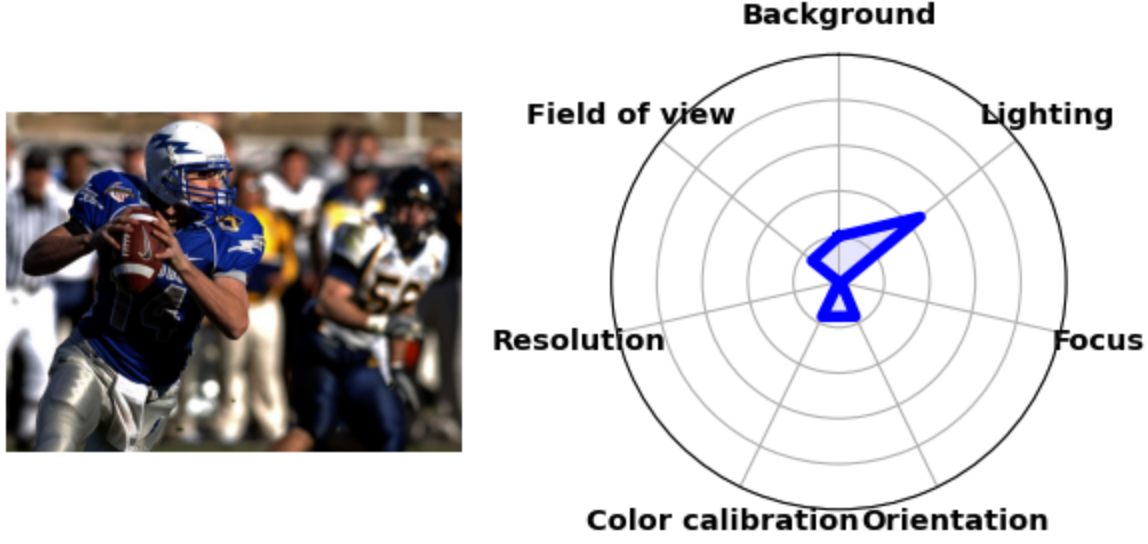
\includegraphics[width=\textwidth]{img/ood/4ll.png}
        \caption{Lighting (Darken)}
        \label{fig:4ll}
    \end{subfigure}

    \begin{subfigure}[b]{0.48\textwidth}
        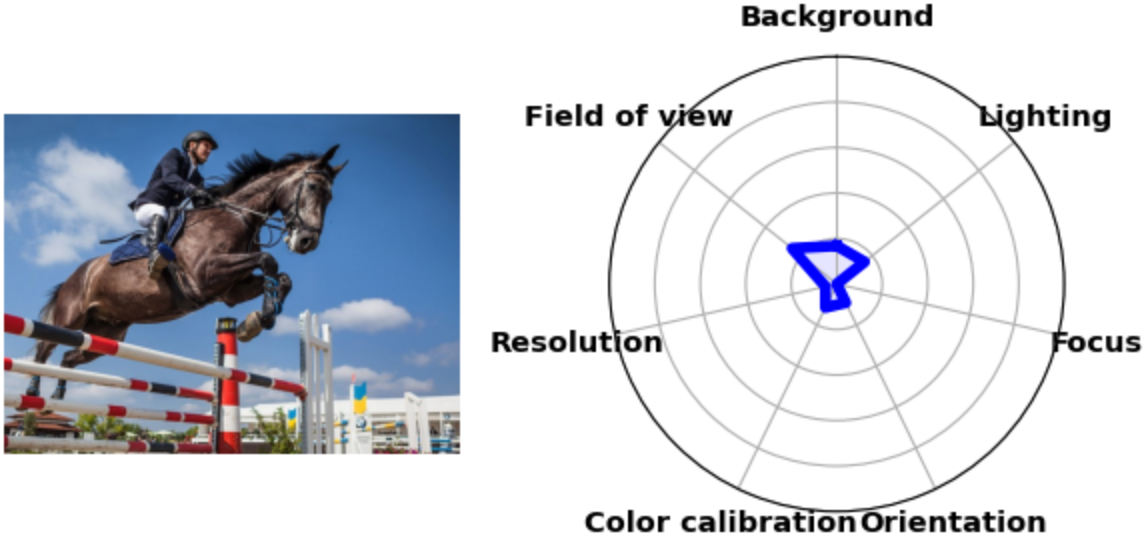
\includegraphics[width=\textwidth]{img/ood/3.png}
        \caption{Good Quality}
        \label{fig:3}
    \end{subfigure}
    \hfill
    \begin{subfigure}[b]{0.48\textwidth}
        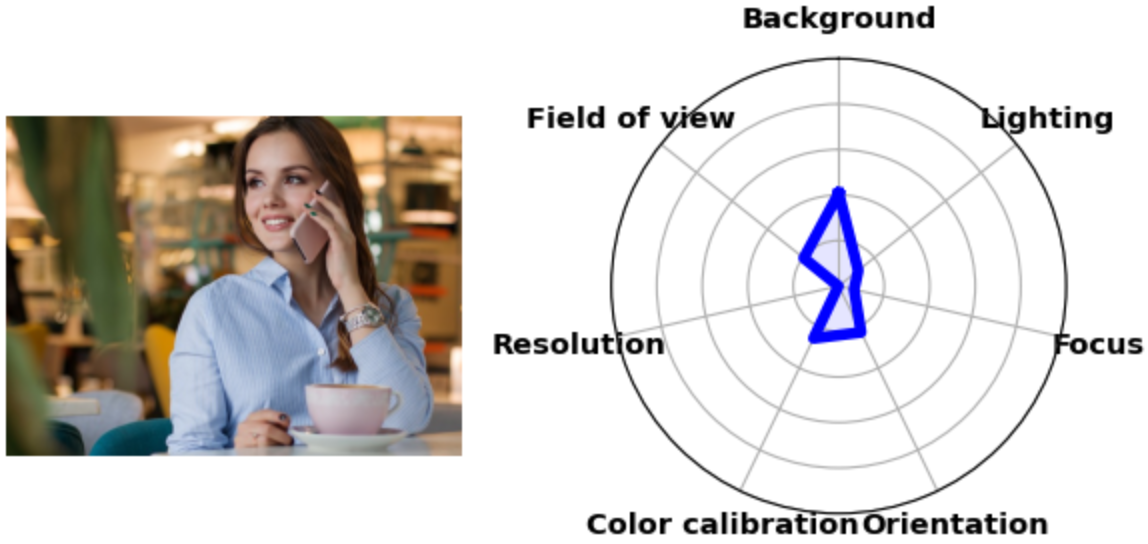
\includegraphics[width=\textwidth]{img/ood/5.png}
        \caption{Good Quality}
        \label{fig:5}
    \end{subfigure}
    \caption{Out of distribution testing with images from the KADID10K dataset.}
    \label{fig:ood1}
\end{figure}

